\section{Validierung}
Um die Forschungsfragen zu beantworten, haben wir die gesammelten Immobiliendaten auf Verwertbarkeit analysiert und gefiltert.\\
Bei den Machine Learning Algorithmen haben wir den MAPE sowie der MdAPE als wichtiges Performanzkriterium genommen. Weiter war uns wichtig, wie viele Inserate können mit einer Abweichung von 10\% geschätzt werden.\\
Gewisse Daten haben so extreme Werte, dass sie die Diagramme verzerren und so eine Aussage über die Daten erschweren. Deshalb werden diese Werte für die Validation ignoriert. Dabei handelt es sich um insgesamt 751 Inserate. Weiter wurden 12’219 Inserate weggelassen, da bei diesen der Kaufpreis fehlte.
Im nächsten Kapitel wird der Iterative Vorgang beschrieben.
%
\subsection{Gesammelte Daten}
Insgesamt konnten 162’225 Immobilieninserate in einem Zeitraum von 5 Monaten gesammelt werden. Davon stammen die meisten vom Immoscout24 Portal, was in Tabelle \ref{tab:crawled_data} ersichtlich ist.
\begin{table*}[ht]
\centering
\ra{1.3}
\begin{tabular}{@{}lrr@{}}
\toprule
Portal & Anzahl gesammelte Inserate & Anzahl verwendete Inserate \\
\midrule
Immoscout & 94'611 & 46'226\\
Homegate & 34'115 & 19'568\\
Newhome & 32'600 & 19'011\\
Urbanhome & 2'047 & 1'040\\
\bottomrule
\end{tabular}
\caption{Auswertung der gesmmelten Daten}
\label{tab:crawled_data}
\end{table*}
%
Von den insgesamt 162’225 Inseraten wurden 77’608 ungültige Inserate herausgefiltert. 
Dabei handelte es sich mehrheitlich um fehlerhafte Inserate oder Inserate, bei denen wichtige Kennwerte fehlten.\\
Insgesamt konnten 83’107 Wohungen und 65’430 Häuser gesammelt werden. Die restlichen Inserate waren Lagerräume oder nicht definierte Immobilientypen.\\
Weiter konnte für 83\% aller Inserate, mit einer vollständigen Adresse eine Lärmbelastung berechnet werden. Ebenso konnten für 99\% aller Inserate eine Gemeinde zugeordnet werden.\\
Die meisten Inserate haben eine Angabe über die Anzahl Zimmer und Wohnfläche. Gefolgt vom Baujahr und der Anzahl an Stockwerken, falls es mehrere besitzt. Die Raumhöhe oder die Kubatur wird dagegen nur selten angegeben. So auch die effektive Fläche einer Immobilie. Abbildung \ref{fig:features} zeigt den prozentualen Anteil der fehlenden Kennwerte.\\[2ex]
\begin{figure}[h!]
\centering
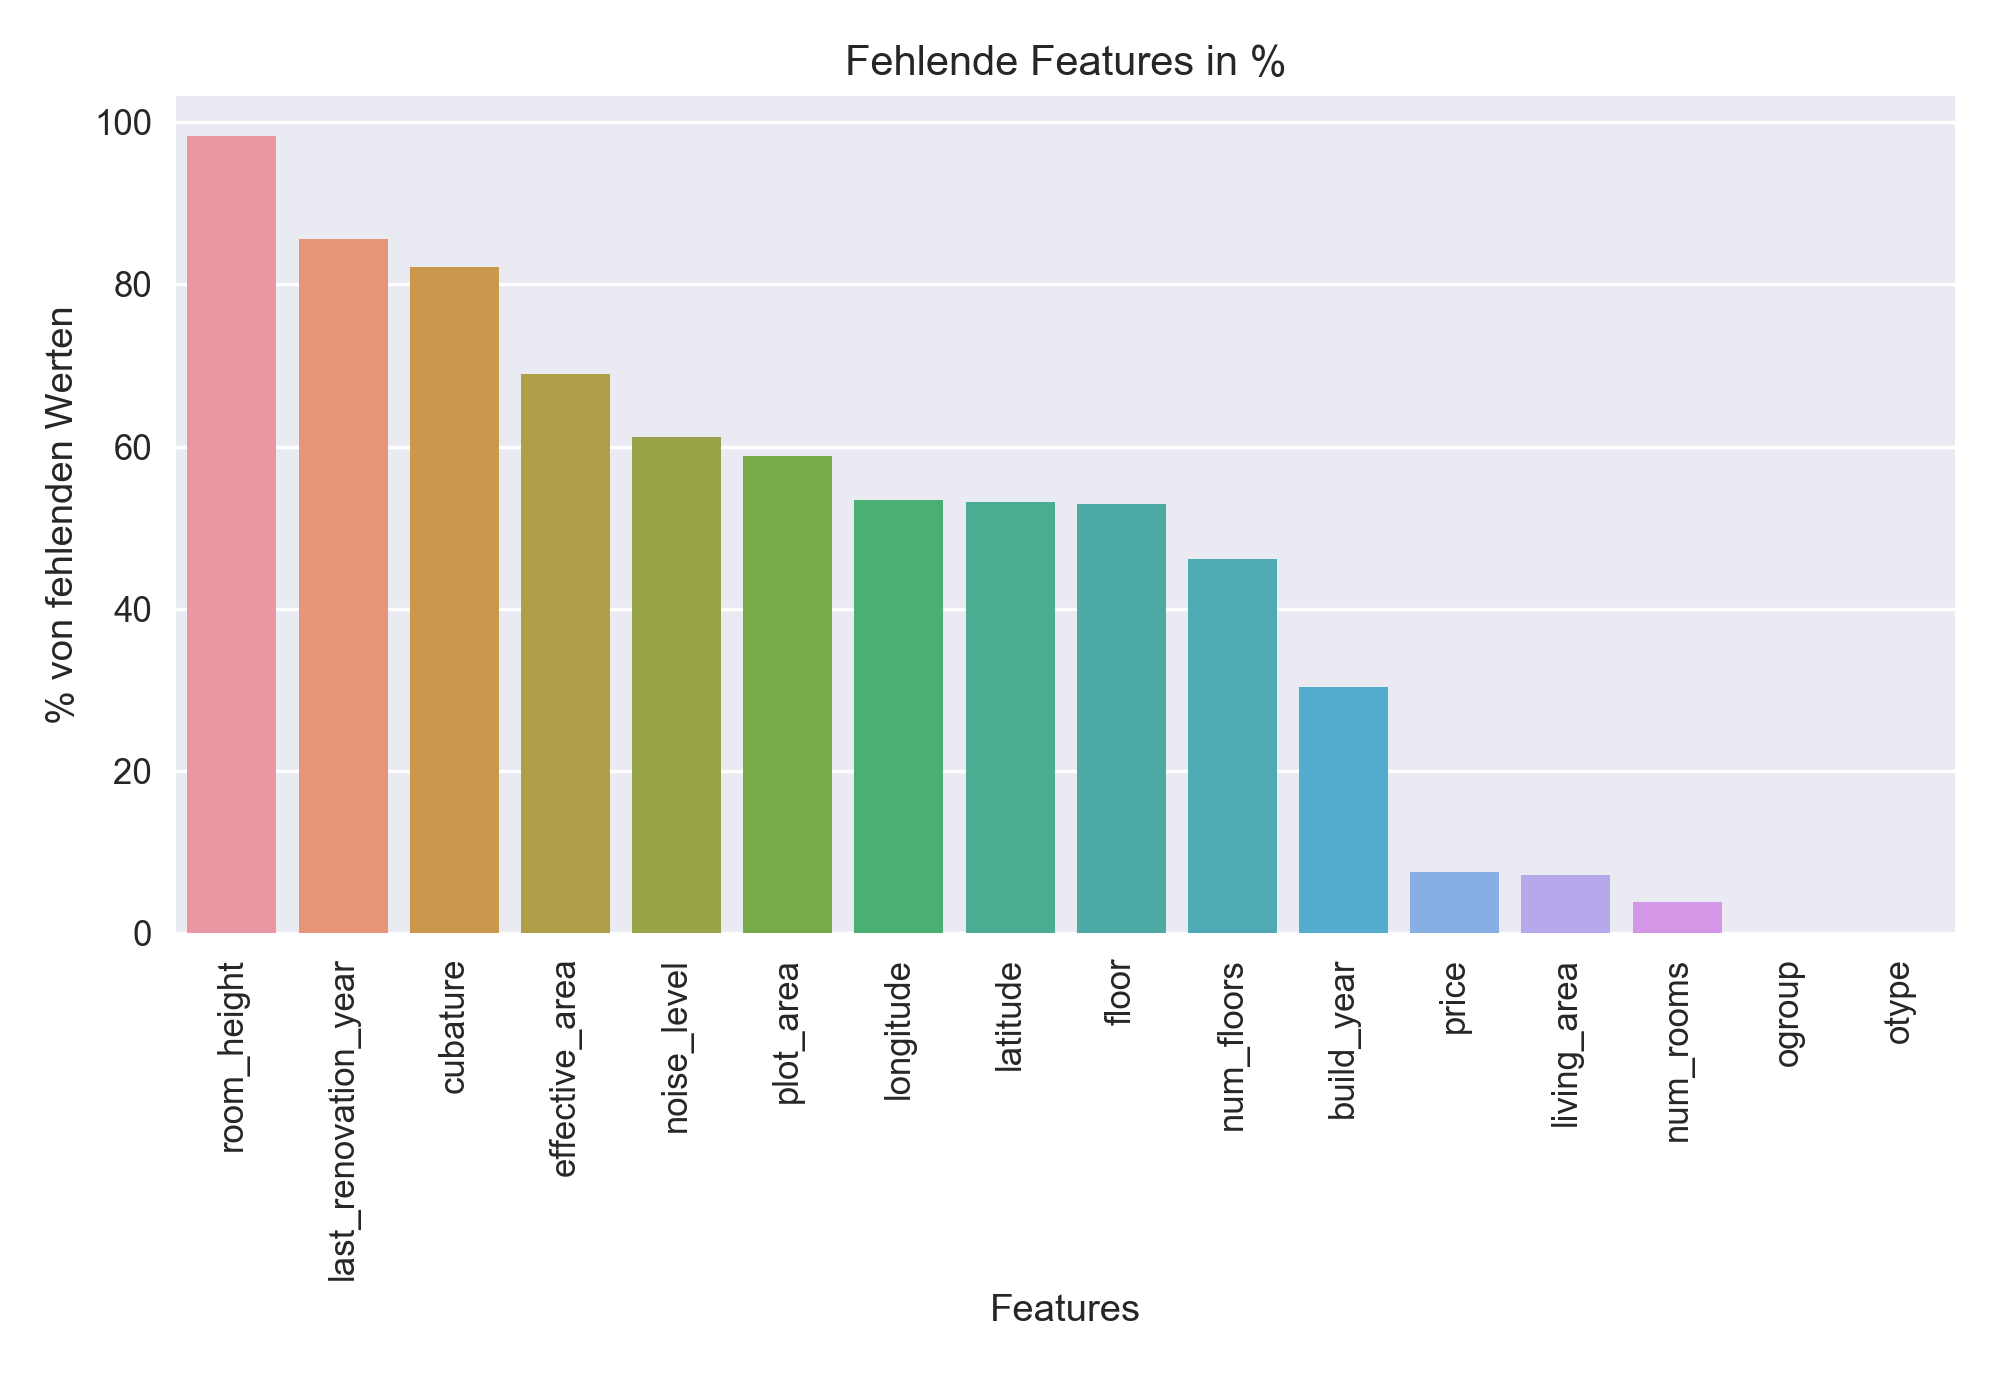
\includegraphics[width=0.9\textwidth]{images/missing_values.png}
\caption[Anzahl der vorkommenden Features]{Anzahl der vorkommenden Features}%
\label{fig:features}
\end{figure}
\newline
%
Die Crawler wurden nie über eine längere Zeit gesperrt. Vereinzelt kam es zu Blockierungen, die jedoch, durch das Starten neuer Proxyinstanzen, umgehen werden konnten. Der Zeitaufwand um ein Portal bei fünf gleichzeitigen Verbindungen und einer Download Delay von zwei Sekunden zu crawlen, lag im Schnitt bei 4 Stunden. Dementsprechend wurden in dieser Zeit etwa 100 Proxyinstanzen gestartet.\\[2ex]
%
Die Datenqualität ist eher mässig, da viele Inserate erst gar nicht für ein Trainingsdatensatz verwendet werden können. Um dem entgegenzuwirken, wurde versucht durch Feature Engineering fehlende Daten zu berechnen.
%
\subsubsection{Kaufpreis}
Abbildung \ref{fig:price} zeigt die Verteilung des Kaufpreises. Dabei sieht man, dass dieser nicht normalverteilt ist (\ref{fig:price_normal}). Es besteht eine positive Skenwess, was für eine Lineare Regression nicht optimal ist. Wird der Log-Wert des Preises genommen (\ref{fig:price_log}), kann eine Annäherung an eine Normalverteilung erreicht werden. Dies gilt es zu beachten, wenn später mit einer Linearen Regression gearbeitet wird.
Tabelle \ref{tab:price} zeigt die beschreibenden statistischen Werte des Preises.
%
\begin{figure}[ht]
\begin{subfigure}{.5\textwidth}
  \centering
  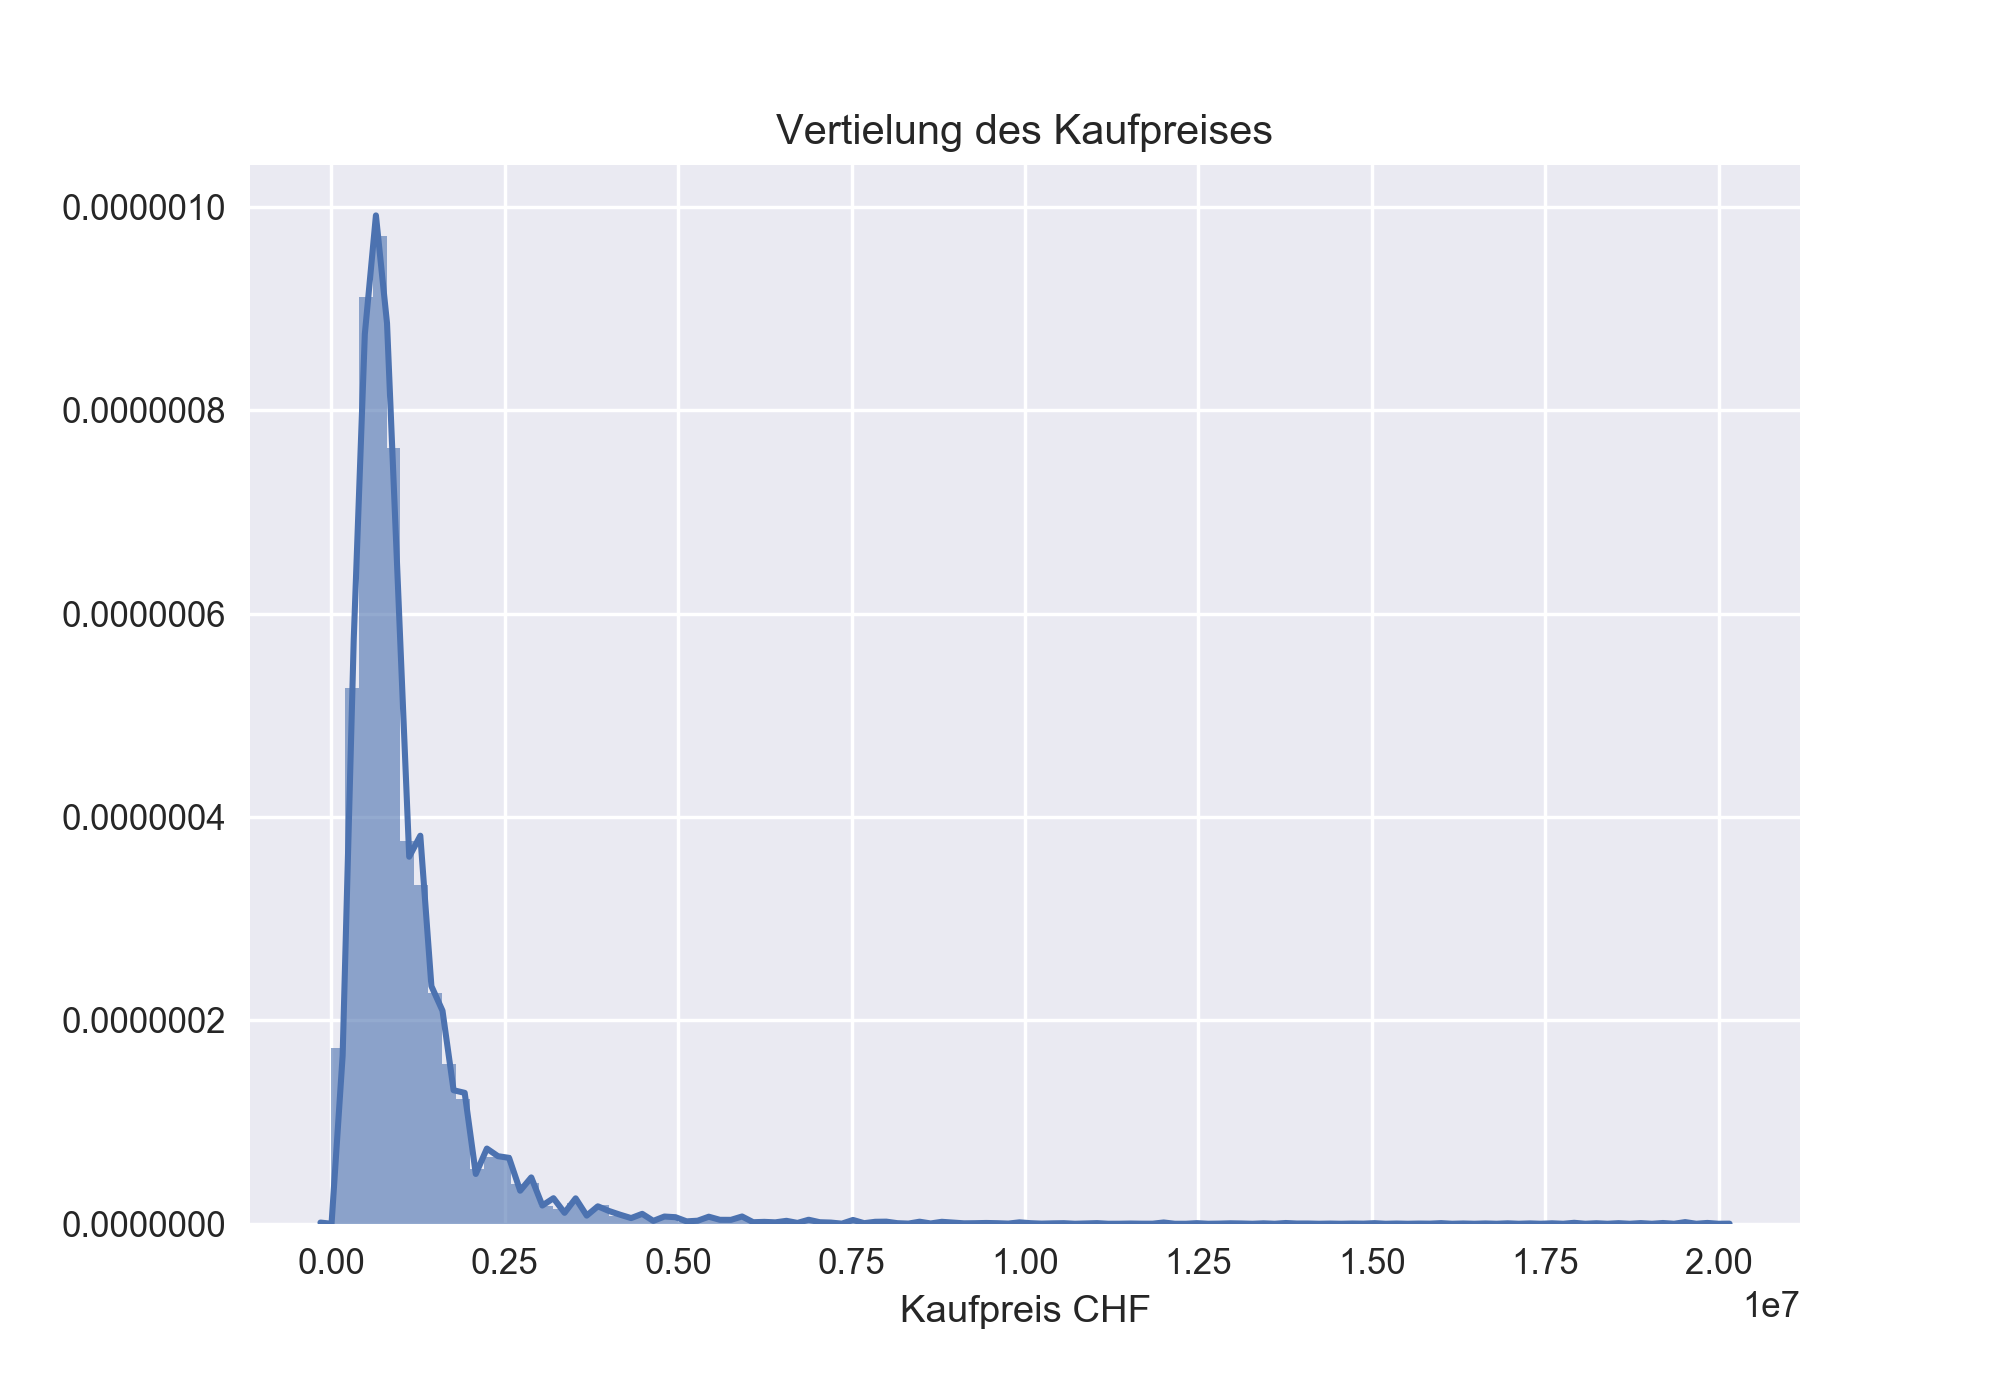
\includegraphics[width=\linewidth]{images/Verteilung_des_kauf_preises.png}
  \caption[Verteilung des Kaufpreises aller Immobilien]{Verteilung des Kaufpreises aller Immobilien}
  \label{fig:price_normal}
\end{subfigure}%
\begin{subfigure}{.5\textwidth}
  \centering
  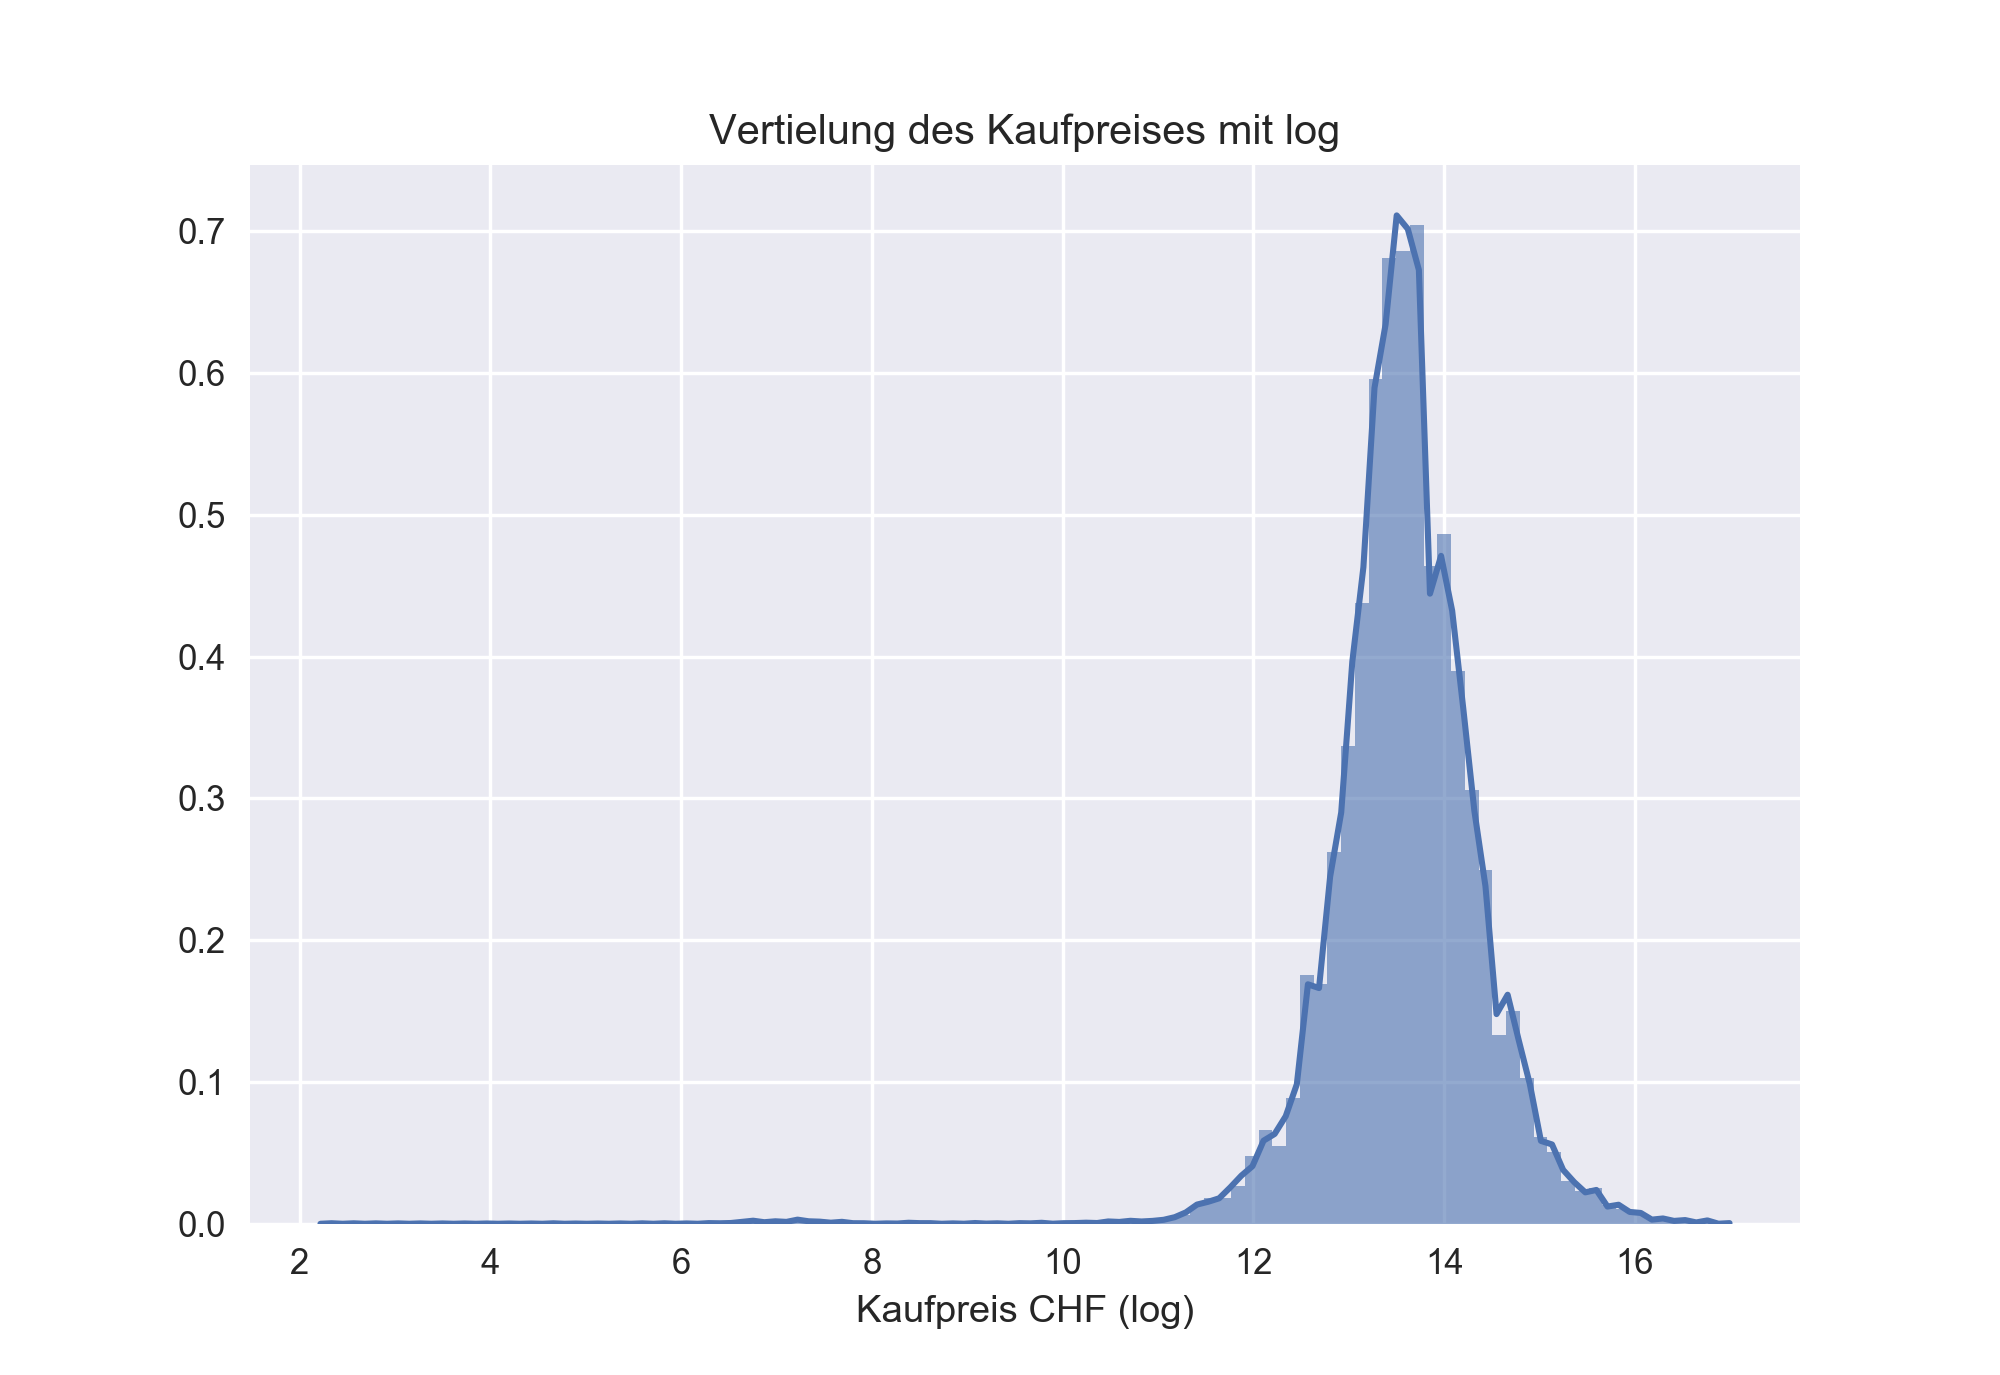
\includegraphics[width=\linewidth]{images/Verteilung_des_kauf_preises_log.png}
  \caption[Verteilung des Log(Preises)]{Verteilung des Log(Preises)}
  \label{fig:price_log}
\end{subfigure}
\caption[Kaufpreis analyse: Verteilung]{Kaufpreis analyse: Verteilung}
\label{fig:price}
\end{figure}
%
\begin{table*}[ht]
\centering
\ra{1.3}
\resizebox{\textwidth}{!}{
\begin{tabular}{@{}lrrrrr@{}}
\toprule
 & Min & Max & Durchschnitt & Median & Standardabweichung\\
\midrule
Preis: Haus & 10 & 20'000'000 & 1'281'735 & 920'000 & 1'309'085\\
Preis: Wohnung & 10 & 20'000'000 & 891’479 & 690’000 & 786’047\\
Pries: Alle & 10 & 20’000'000 & 1’059’503 & 790’000 & 1’066’372\\
\bottomrule
\end{tabular}}
\caption{Statistische Werte des Kaufpreises}
\label{tab:price}
\end{table*}
%
\subsubsection{Numerische Features}
Bis auf die Lärmbelastung wurden alle numerischen Features von Inseraten gesammelt.\\
Abbildung \ref{fig:num_features} zeigt einen Teil dieser Features in Verbindung zum Kaufpreis. Dabei ist ersichtlich, dass die Wohnfläche, Kubatur und Anzahl Zimmer eine linear ähnliche Abhängigkeit haben. Beim Rest ist eher unklar, wie sie zum Preis stehen.\\[2ex]
%
\begin{figure}[h!]
\centering
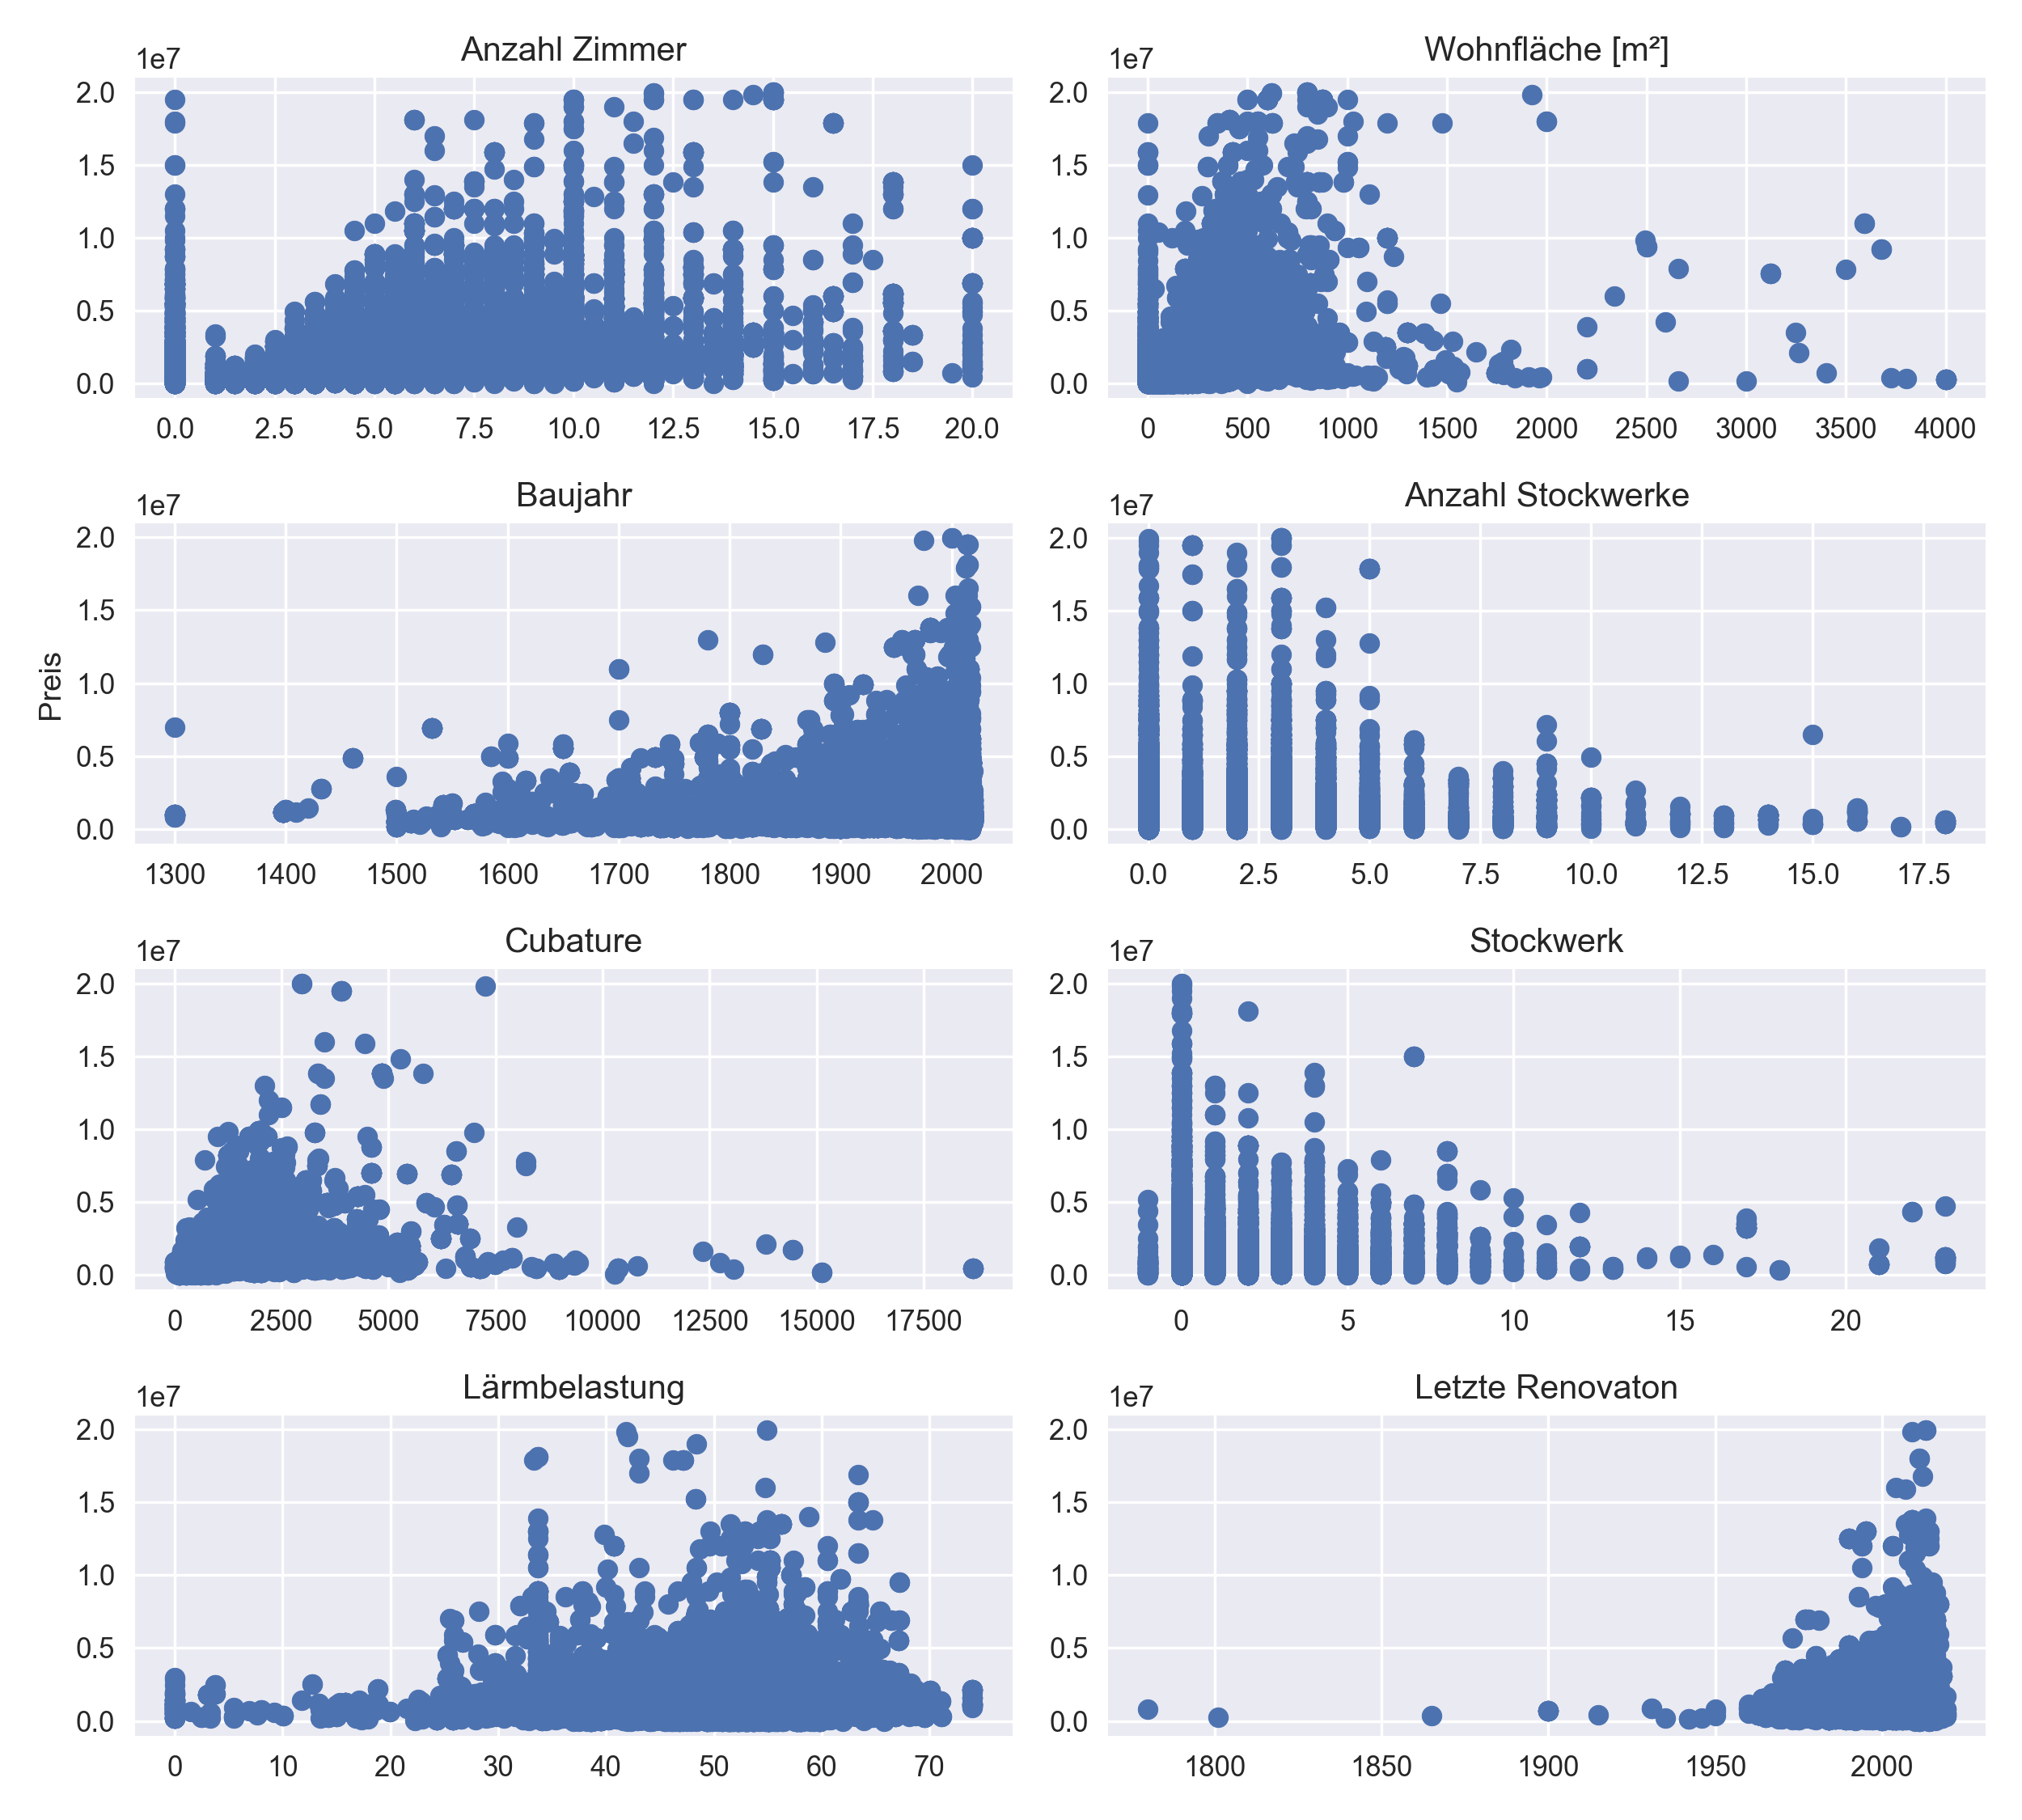
\includegraphics[width=0.9\textwidth]{images/Vergleich_zum_preis.png}
\caption[Nummerische Feature im Vergleich zum Preis]{Nummerische Feature im Vergleich zum Preis}%
\label{fig:num_features}
\end{figure}
\newline
%
Tabelle \ref{tab:num_features} zeigt die statistischen Werte für die numerischen Features. Die gesammelten Kennwerte sehen plausibel aus und decken sich zum Teil mit den Daten vom Bundesamt für Statistik\footnote{https://www.bfs.admin.ch/bfs/de/home/statistiken/bau-wohnungswesen.html}.\\
Auffallend ist, dass der Durchschnitt und der Median bei vielen Features sehr nahe beieinander liegen. Somit gleicht die Verteilung einer Normalverteilung.\\
Einzig störend sind die 0-Werte bei den Features Anzahl Zimmer und Fläche. Diese sollte wenn möglich weitgehend herausgefiltert werden.\\[2ex]
%
\begin{table*}[ht]
\centering
\ra{1.3}
\resizebox{\textwidth}{!}{
\begin{tabular}{@{}lrrrrr@{}}
\toprule
 & Min & Max & Durchschnitt & Median & Standardabweichung\\
\midrule
Anz. Zimmer & 0& 20 & 4.84 & 4.5 & 1.9\\
Fläche & 0 & 4’000 & 143.08 & 130 & 101.924\\
Baujahr & 1300 & 2019 & 1988 & 2006 & 51.52\\
Anz. Stockwerke & 0 & 18 & 1.8 & 2 & 1.747\\
Kubatur & 1 & 18649 & 1059.74 & 867 & 838.419\\
Stockwerk & -1 & 23 & 1.25 & 1 & 1.57\\
Lärmbelastung & 0 & 73.99 & 48.8 & 49.35 & 6.85\\
Letzte Renovation & 1780 & 2019 & 2009 & 2012 & 9.09\\
\bottomrule
\end{tabular}}
\caption{Statistische Werte der nummerischen Features}
\label{tab:num_features}
\end{table*}
%
Abbildung \ref{fig:heatmap} zeigt eine Heatmap der einzelnen Features. Sie zeigt, welche Features stark untereinander korrelieren. Folglich demonstriert sie von welchen Features der Preis abhängig ist. Somit sollte wenn möglich alle Features, die eine hohe Korrelation mit dem Kaufpreis besitzen, ins Modell miteinbezogen werden.
%
\begin{figure}[h!]
\centering
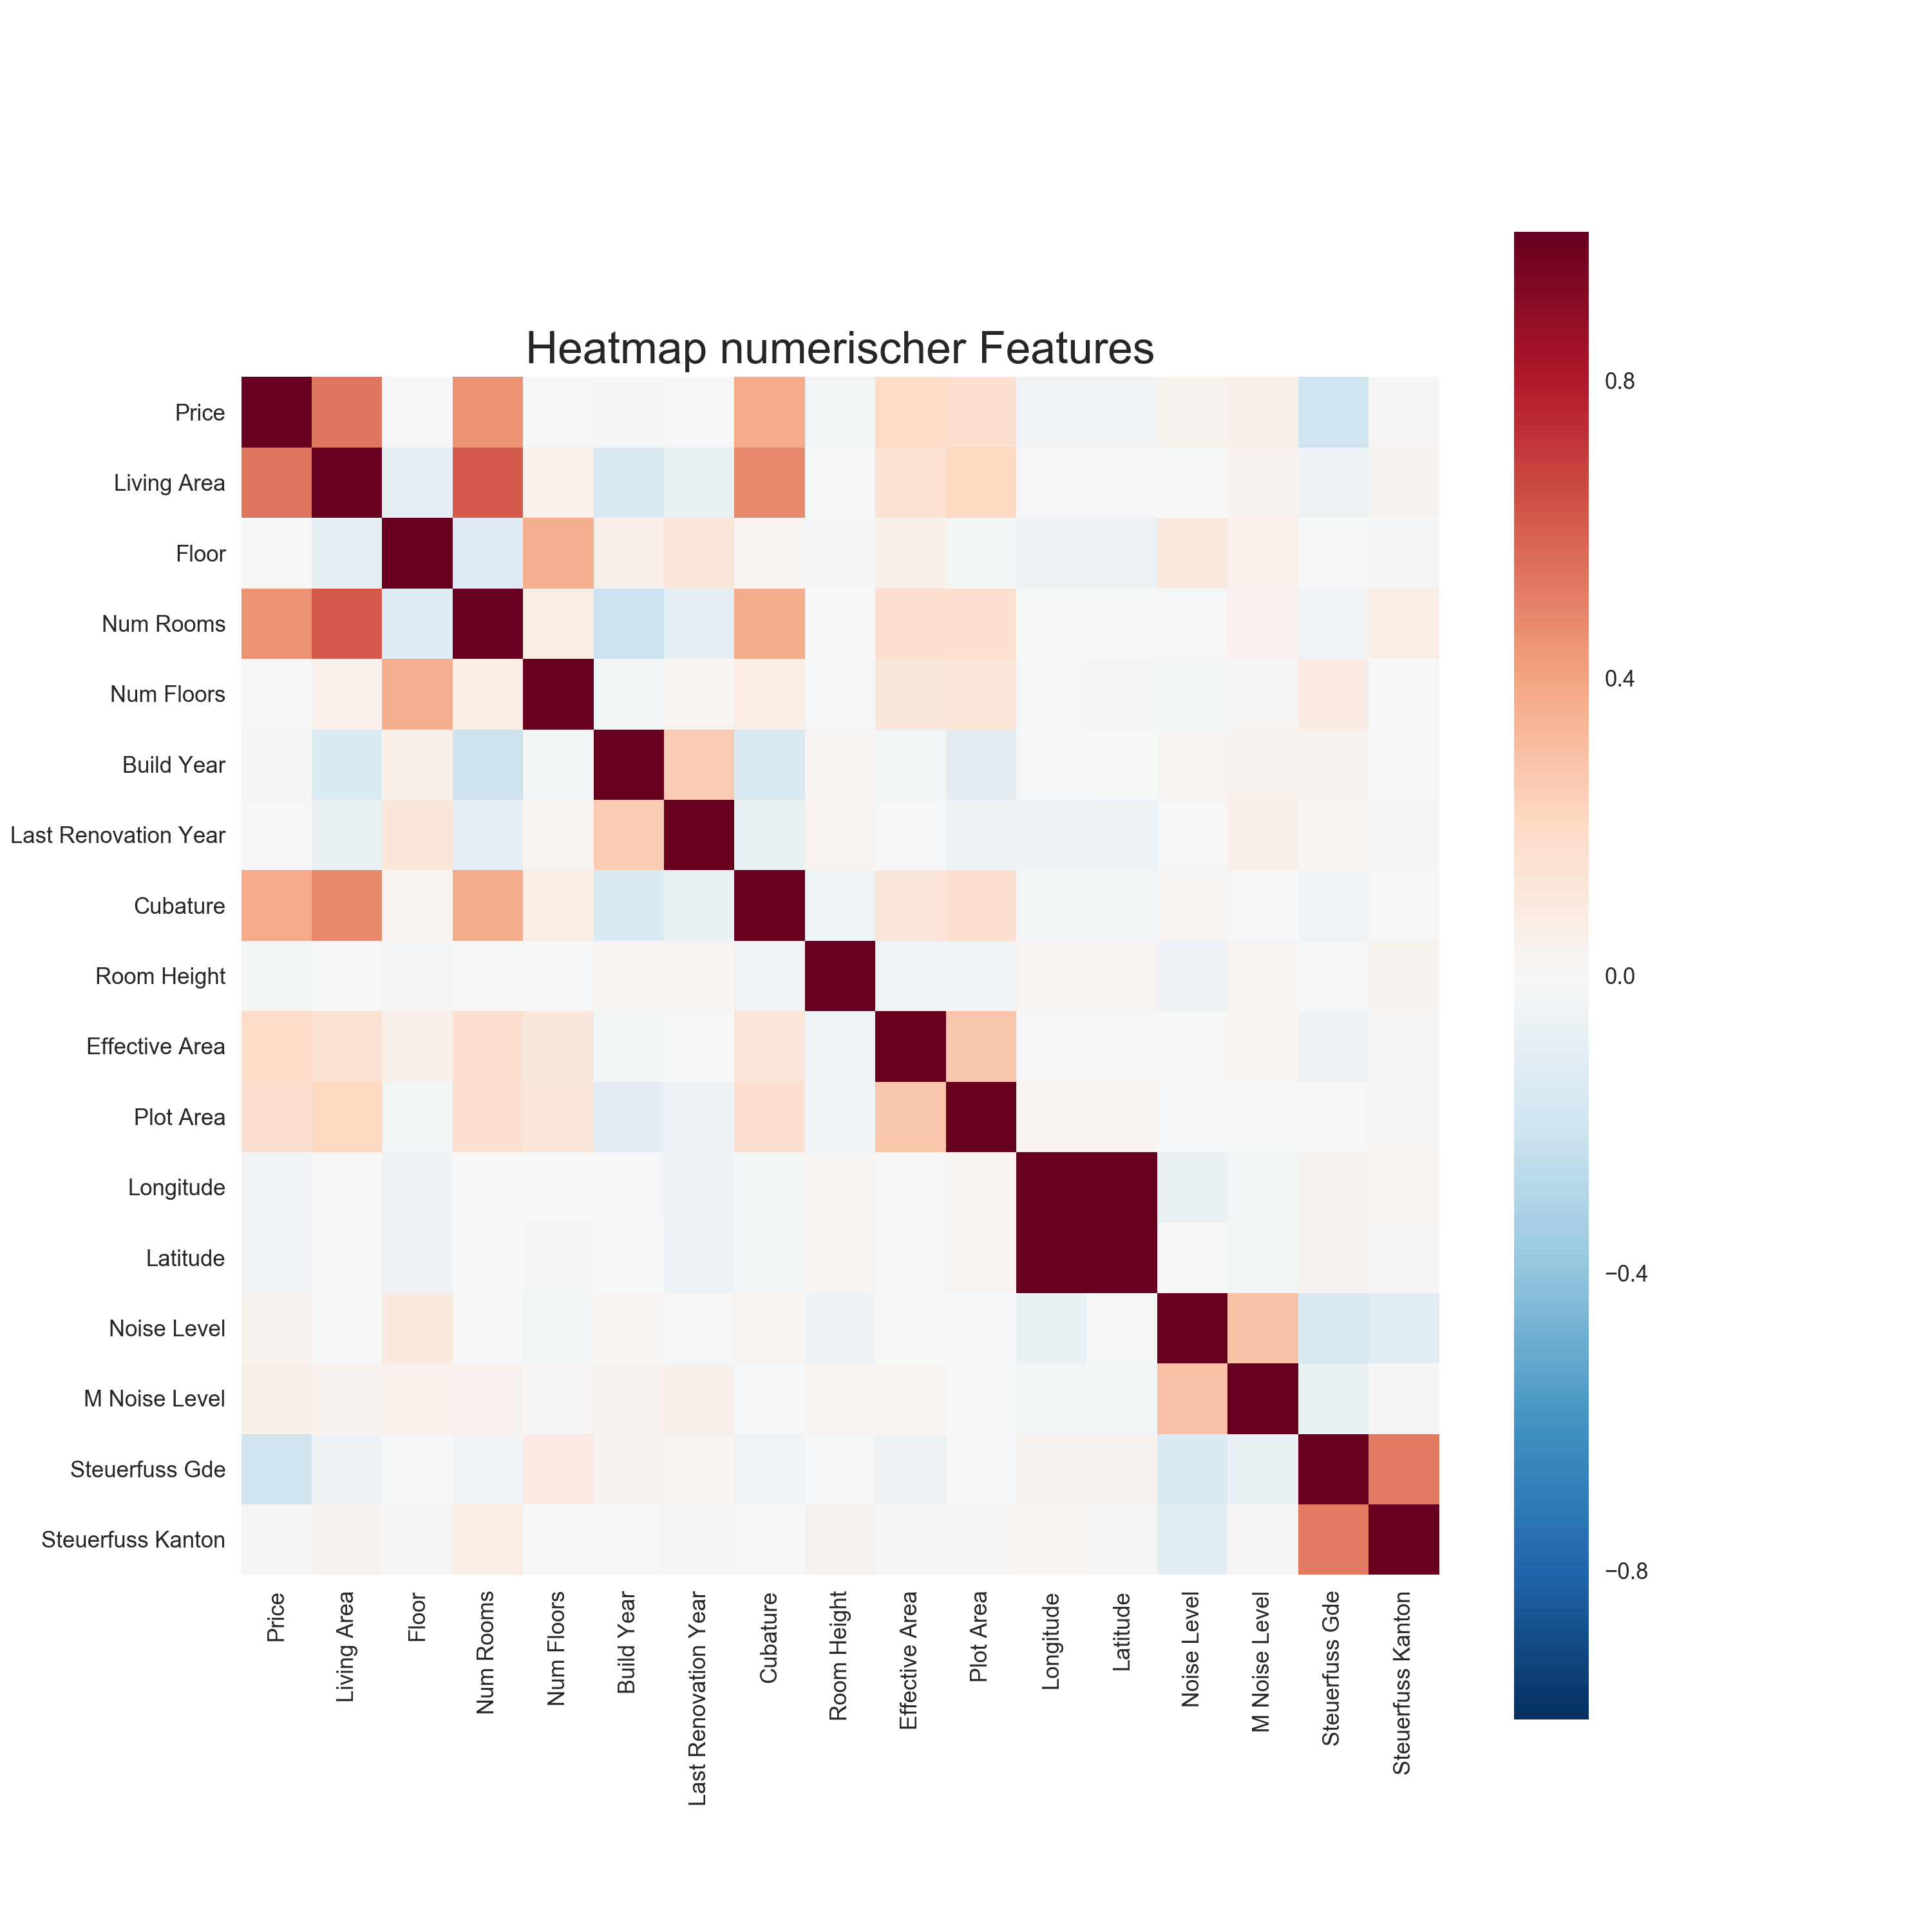
\includegraphics[width=0.9\textwidth]{images/Heatmap_numerical.png}
\caption[Heatmap der nummerischen Features]{Heatmap der nummerischen Features}%
\label{fig:heatmap}
\end{figure}
\newline
%
\subsubsection{Kategorische Features}
Bei den Kategorischen Features handelt es sich vor allem um ortsbezogene Features. Viele davon beschreiben die Region, indem sich die Immobilie befindet.\\
Insgesamt wurden 35 kategorische Features verwendet. Eine Analyse der ortsbezogenen Features mit dem Kaufpreis ergab keine unerwarteten Ergebnisse. So zeigt sich, dass der Kanton Genf die teuersten Immobilien in der Schweiz besitzt, gefolgt von Zug. Abbildung \ref{fig:cantons}.
Auch wurde ersichtlich, dass städtische Immobilien im Schnitt teurer sind als auf dem Land, beziehungsweise je urbaner die Region, desto teurer der Immobilienpreis. Weiter ist ersichtlich, dass  ein Haus im Schnitt mehr kostet als eine Wohnung.\\[2ex]
\begin{figure}[ht]
\centering
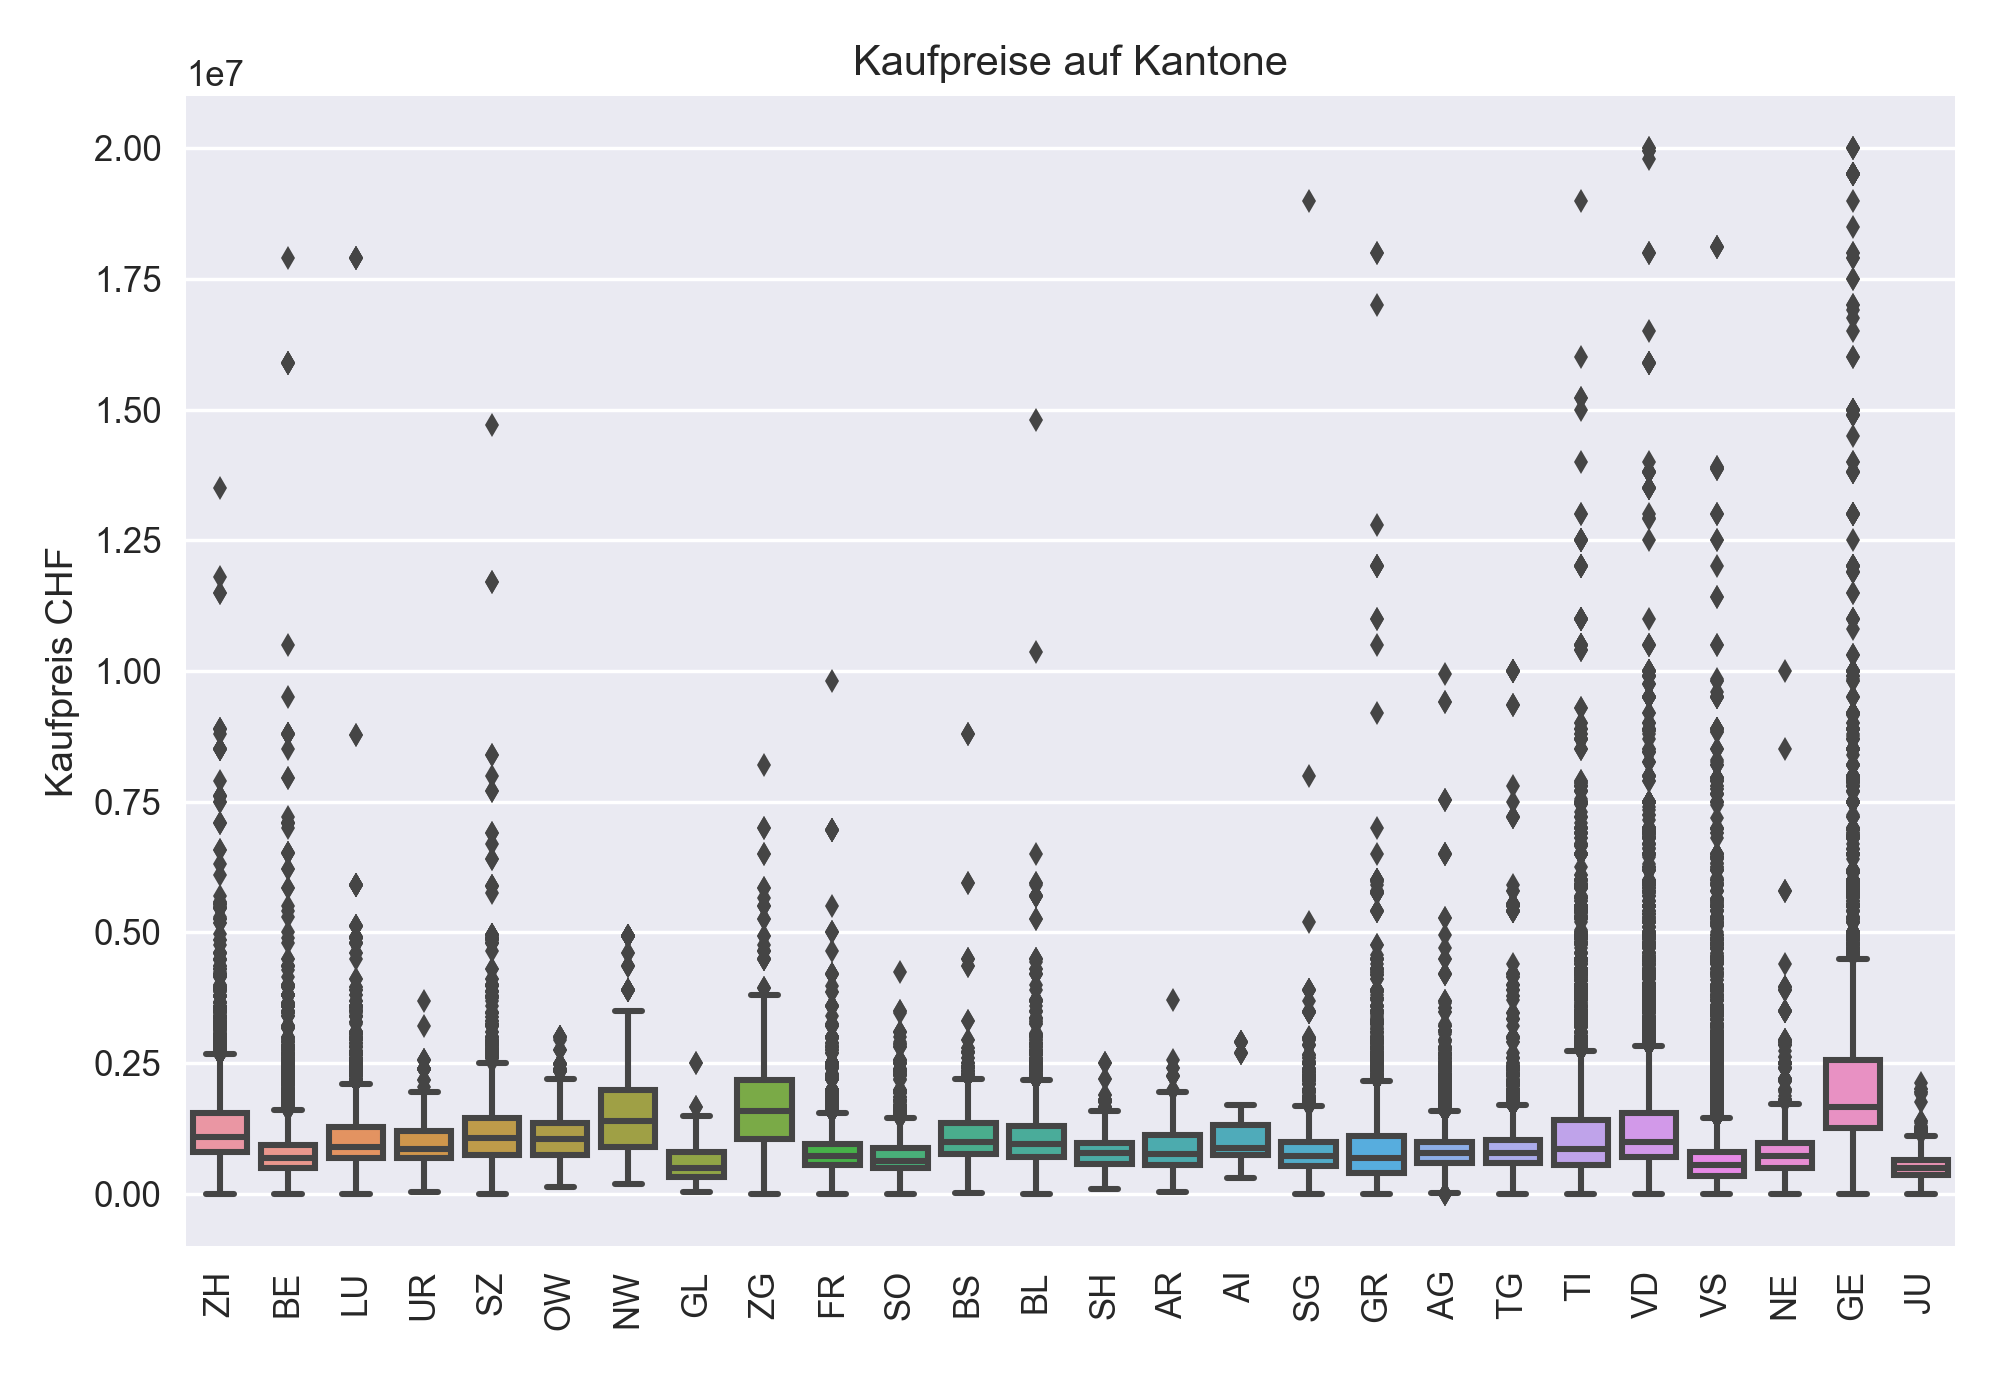
\includegraphics[width=\textwidth]{images/boxPlot_cantons.png}
\caption[Kaufpreis auf Kantonte aufgeteilt]{Kaufpreis auf Kantonte aufgeteilt}%
\label{fig:cantons}
\end{figure}
\newline
%
\textbf{Beschreibung / Charakteristik}
Weitere charakteristische Features stammen aus der Beschreibung und Merkmal analyse. Die 50 häufigsten vorkommenden Wörter die in unserem Datensatz vorkommen, werden in Abbildung \ref{fig:tags} gezeigt. 
\begin{figure}[ht]
\centering
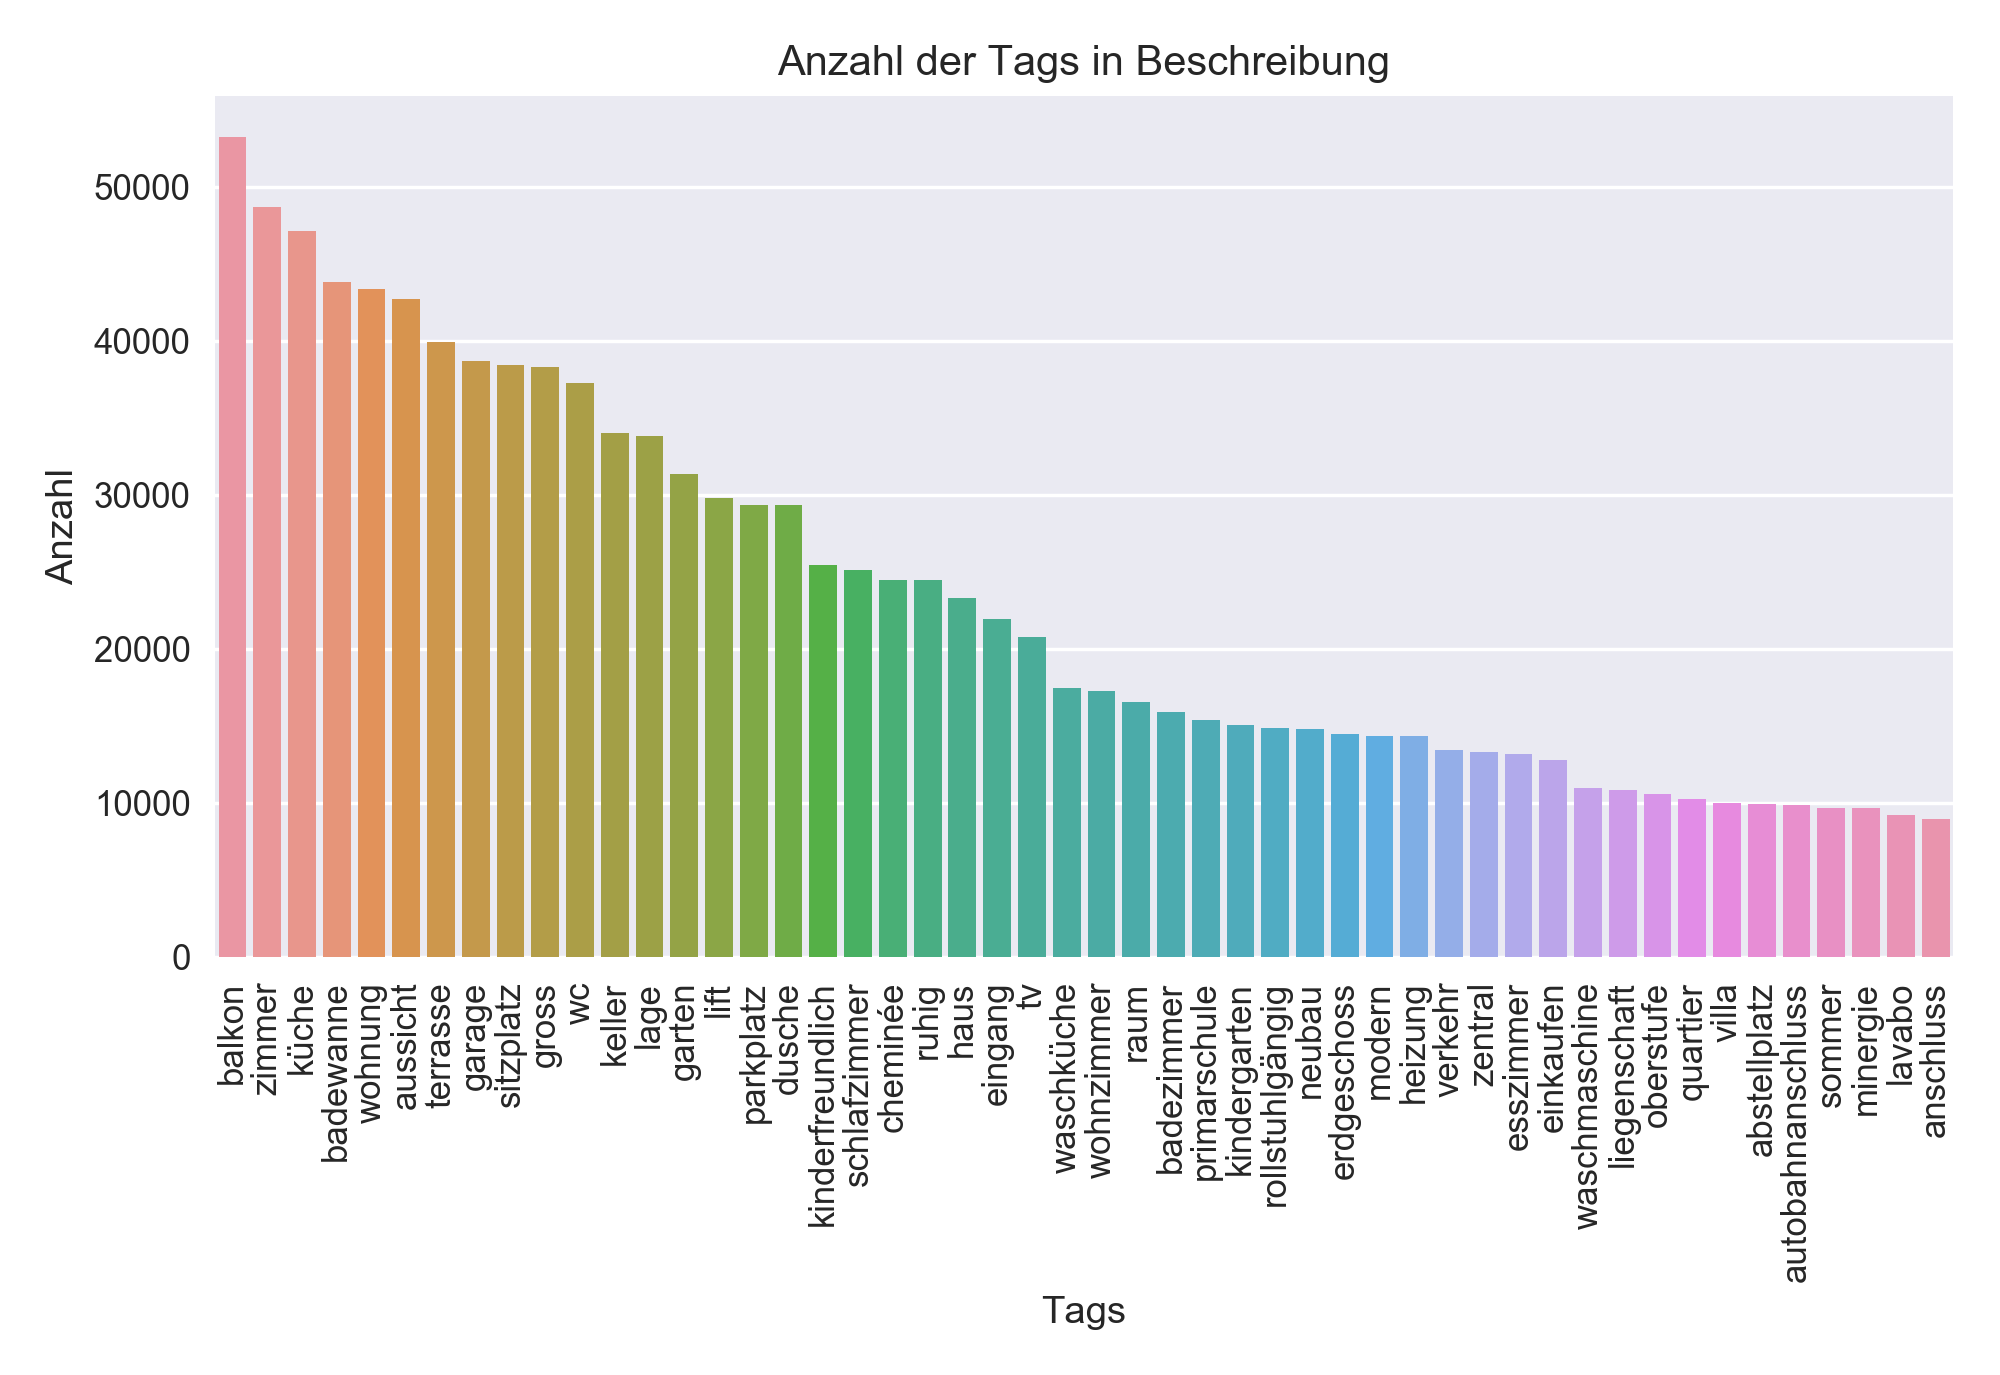
\includegraphics[width=\textwidth]{images/tags.png}
\caption[Häufigkeit der gefundenen Tags]{Häufigkeit der gefundenen Tags}%
\label{fig:tags}
\end{figure}
\newline
%
\subsection{Machine Learning}
Insgesamt haben wir neun verschiedene Machine Learning Algorithmen untersucht. Um eine faire Bewertung zu bekommen, bekamen alle Algorithmen die gleichen Datensätze zum Trainieren wie auch zum Testen. So wurde verhindert, dass ein Algorithmus anhand eines guten Datensatzes eine bessere Performance erzielte.\\[2ex]
%
Damit wir unsere gesammelten Daten für die Algorithmen verwenden können, müssen diese, wenn nötig, richtig transformiert werden. Dafür wird Feature Engineering angewendet, das nach und nach erweitert und verbessert wird.\\[2ex]
%
Als Basis für unsere Feature Engineering Pipeline transformieren wir unseren kategorischen Features mit Hilfe einer One-Hot-Encoding in binäre Features um. So konnten aus 35 Features über 2000 Features gewonnen werden.\\
Es ist nicht möglich alle gesammelten Features zu verwenden. Der Grund ist, dass gewisse Features nur bei wenigen Inseraten angegeben wurden. Wie im vorherigen Kapitel gezeigt, sind dies die Features Kubatur, Raumhöhe, effektive Fläche, Grundstücksfläche, Anzahl Stockwerke, Stockwerk und Renovationsjahr.\\
Als letzter Schritt werden die Inserate gelöscht, die keinen Eintrag bei einem verwendeten Feature besitzen oder doppelt vorkommen. Verwendet werden schlussendlich: Wohnfläche, Anzahl Zimmer, Baujahr Renovationsjahr, die Beschreibung und die Merkmale.
%
\subsubsection{Regressions Algorithmen}
Für die Auswertung der Algorithmen starten wir mit den Regressions Algorithmen. Hierfür verwenden wir eine  einfache lineare Regression, den Ridge- und Lasso-Algorithmus. Die Ergebnisse werden in Tabelle \ref{tab:regression} angezeigt.\\[2ex]
%
\begin{table*}[ht]
\centering
\ra{1.3}
\resizebox{\textwidth}{!}{
\begin{tabular}{@{}lrrrrr@{}}
\toprule
ML Algorithmus & $R^2$ & MAPE & MdAPE & 10\% Abweichung & Maximaler Fehler\\
\midrule
Lineare Regression & -4.26E+25 & 2.93322E+13 & 21.793 & 25.029 & 5.81E+20\\
Ridge Regression & 0.329459 & 61.722 & 28.824 & 19.005 & 2.87E+07\\
Lasso Regression & 0.57609 & 70.044 & 19.458 & 27.823 & 2.71E+07\\
\bottomrule
\end{tabular}}
\caption{Ergebnisse der Regression Algorithmen}
\label{tab:regression}
\end{table*}
%
Wir sehen, dass die Algorithmen eher schlecht abschneiden. Zum Einen liegt das daran, dass noch kein richtiges Feature Engineering durchgeführt wurde. Zum Anderen haben wir sehr viele kategorischen Features in unserem Modell. Die Lineare Regression erwartet eine Normalverteilung der Features, was bei Kategorischen nicht der Fall ist. Wie oben angemerkt, kann eine Verbesserung erzielt werden, wenn der Log-Wert des Preises verwendet wird.\\
Es ist ersichtlich, dass die Algorithmen mit einem Regularisierungsparameter eine deutlich bessere Performance erzielen, als eine normale lineare Regression. Somit ist ein Regularisierungsparameter bei über 2000 Features, der ein Overfit verhindert und somit die Komplexität reduziert, nützlich.\\
Auffallend ist, dass der Lasso Algorithmus eine deutliche bessere Performance hat als der Ridge Algorithmus vorweist. Dies kann auf ein schlechtes Feature Engineering zurückgeführt werden. Denn der Lasso kann unnötige Features eliminieren, während der Ridge alle Features verwendet.
%
\subsubsection{K-Nearest Neighbour}
Beim nächsten Algorithmus handelt es sich um den K-Nearest Neighbour. Dieser Algorithmus versucht anhand der Nachbarn den Preis zu schätzen. Der Vorteil gegenüber den Regressions Algorithmen ist, dass es dem Algorithmus egal ist, in welchem Format die Features vorhanden sind. Zudem haben viele Features keinen negativen Einfluss auf den Algorithmus.
Tabelle \ref{tab:kneighbour} zeigt die erzielten Resultate des Algorithmus der zwei Nachbarn zum Vergleich verwendete und eine Leaf size von 100 hatte. Für die Gewichtung wurde ein Euklid-Distanz genommen.\\[2ex]
%
\begin{table*}[ht]
\centering
\ra{1.3}
\resizebox{\textwidth}{!}{
\begin{tabular}{@{}lrrrrr@{}}
\toprule
ML Algorithmus & $R^2$ & MAPE & MdAPE & 10\% Abweichung & Maximaler Fehler\\
\midrule
K-Nearest Neighbour & 0.830364 & 23.673 & 0 & 79.941 & 1.81E+07\\
\bottomrule
\end{tabular}}
\caption{Ergebnisse vom K-Nearest Neighbour}
\label{tab:regression}
\end{table*}
%
Die Performance ist deutlich besser als bei den Regressions Algorithmen. 77,45\% der Immobilien können mit einer Abweichung von 10\% richtig geschätzt werden. Das zeigt anhand diesem Algorithmus auf, dass bei ähnlichen Immobilien auch ein ähnlicher Preis existieren muss.\\
Eine MdAPE von 0 erklären wir damit, dass es sehr ähnliche Häuser gibt, die den selben Preis besitzen. Das kann vorkommen, wenn neue Reihenhäuser oder ein neuer Wohnungsblock inseriert wird. Die MAPE mit einem Wert von 26,86\% ist jedoch zu hoch um von einem guten Modell zu sprechen.\\[2ex]
%
\subsubsection{Baum Algorithmen}
Als nächstes untersuchen wir verschiedene Baum-Algorithmen. Baum Algorithmen erfreuen sich aktuell einer grosser Beliebtheit bei diversen Machine Learning Wettbewerben\footnote{https://www.kaggle.com/c/house-prices-advanced-regression-techniques}.\\[2ex]
%
Wir haben uns vier verschiedene Algorithmen ausgesucht. Sie unterscheiden sich hauptsächlich in ihrer Strategie. Der Random Forest wendet eine Art Bagging an. Der XGBoost wie auch der AdaBoost verwenden eine Boostingstrategie. Und der Extra Tree verwendet weder ein Boosting noch ein Bagging.\\
Für den Random Forest verwendeten wir bis auf die 700 Schätzungsmodelle die Default Parameter. Dasselbe galt auch für den Extra Tree Algorithmus.\\
Für den AdaBoost haben wir als Basis Schätzungsmodell den DecisionTreeRegressor mit 18 Schätzungsmodelle genommen.\\
Der XGBoost besitzte eine maximale Tiefe von 100 mit einer Lernrate von 0.1 und 350 Schätzungsmodelle.
Die Resultate werden in Tabelle \ref{tab:first_round} dargestellt.\\[2ex]
%
\begin{table*}[ht]
\centering
\ra{1.3}
\resizebox{\textwidth}{!}{
\begin{tabular}{@{}lrrrrr@{}}
\toprule
ML Algorithmus & $R^2$ & MAPE & MdAPE & 10\% Abweichung & Maximaler Fehler\\
\midrule
Random Forest & 0.907 & 23.318 & 2.43 & 77.523 & 1.26E+07\\	
Extra Tree & 0.91 & 23.884 & 0.861 & 81.735 & 1.04E+07\\
XGBoost & 0.898 & 18.712 & 0.809 & 82.014 & 1.46E+07\\
AdaBoost & 0.907 & 18.138 & 0 & 83.692 & 1.63E+07\\
\bottomrule
\end{tabular}}
\caption{Ergebnisse der Baum Algorithmen}
\label{tab:first_round}
\end{table*}
%
Man sieht, dass die Baum Algorithmen, bis auf den Random Forest, eine noch besser Performance haben, als der K-nearest Neighbour. Der AdaBoost kann sogar über 80\% der Inserate mit einer Abweichung von 10\% richtig schätzen. Die vielen kategorischen Features helfen den Baumalgorithmen eine gute Performance zu erzielen. Wie beim K-Nearest Neighbour ist die MAPE noch zu hoch für eine gute Schätzung.\\[2ex]
%
Für das weitere Vorgehen werden nur noch der Extra Tree, XGBoost und der AdaBoost verwendet, da diese die besten Werte erreichten.\\[2ex]
%
Um eine bessere Performance zu erhalten, wird anhand von Feature Engineering versucht weitere Features zu generieren. Aus den beiden Features Wohnfläche und Anzahl Zimmer, berechnen wir die durchschnittliche Zimmergrösse. Wir nehmen diese beiden Features, da diese eine hohe Korrelation mit dem Preis besitzen. Tabelle \ref{tab:second_round} zeigt die Ergebnisse.\\[2ex]
%
\begin{table*}[ht]
\centering
\ra{1.3}
\resizebox{\textwidth}{!}{
\begin{tabular}{@{}lrrrrr@{}}
\toprule
ML Algorithmus & $R^2$ & MAPE & MdAPE & 10\% Abweichung & Maximaler Fehler\\
\midrule
Extra Tree & 0.903292 & 27.144 & 0.818 & 81.426 & 1.76E+07\\
XGBoost & 0.887841 & 25.273 & 0.752 & 81.938 & 2.30E+07\\
AdaBoost & 0.884758 & 23.275 & 0 & 83.971 & 2.33E+07\\
\bottomrule
\end{tabular}}
\caption{Ergebnisse mit durchschnittlicher Zimmergrösse}
\label{tab:second_round}
\end{table*}
%
Die MAPE verschlechterte sich für alle Modelle. Schaut man auf die Gewichtung der einzelnen Features für die Modelle, ist die durchschnittliche Zimmergrösse unter den Top 5. Interessanterweise sind Wohnfläche wie Anzahl Zimmer auch stark gewichtet. Die Gefahr bei stark korrelierenden Features ist, dass sie als ein Feature betrachtet werden. Wird eines der Features verwendet, können die anderen korrelierenden Features an Wichtigkeit verlieren.\\[2ex] 
%
Als nächstes ergänzen wir die bestehenden Features durch ein binäres Feature, das auf 1 steht falls eine Renovation durchgeführt wurde und auf 0 steht falls nicht.\\
Zusätzlich um nicht auf das Renovationsjahr zu verzichten, transformieren wir dieses Feature um. Wir nehmen nicht die Jahreszahl, sondern die Differenz von der Renovation bis Heute. Fehlt das Renovationsjahr, wird für die Differenz das Baujahr genommen.\\
Tabelle \ref{tab:third_round} zeigt das Ergebnis der Modelle.\\[2ex]
%
\begin{table*}[ht]
\centering
\ra{1.3}
\resizebox{\textwidth}{!}{
\begin{tabular}{@{}lrrrrr@{}}
\toprule
ML Algorithmus & $R^2$ & MAPE & MdAPE & 10\% Abweichung & Maximaler Fehler\\
\midrule
Extra Tree & 0.915152 & 20.048 & 0.87 & 81.804 & 8.87E+06\\
XGBoost & 0.910506 & 20.191 & 0.802 & 82.113 & 9.19E+06\\
AdaBoost & 0.920327 & 18.484 & 0 & 83.528 & 9.75E+06\\
\bottomrule
\end{tabular}}
\caption{Ergebnisse mit Einbezug der Renovation}
\label{tab:third_round}
\end{table*}
%
Diese Änderung steigerte die Performance aller Algorithmen. Das zeigt, dass die Renovation eine wichtige Rolle beim Kaufpreis spielt. Die Gewichtung für das binäre Feature, ‘wurde renoviert’ wurde nur schwach gewichtet und hat eine durchschnittliche Gewichtung von 0.2\%. In diesem Fall kann es gut sein, dass dieses Feature durch eine hohe Korrelation mit einem anderen Feature abgeschwächt wird.\\[2ex]
%
Das Bundesamt für Umwelt stellt die Lärmdatenbank sonBASE\footnote{https://www.bafu.admin.ch/dam/bafu/de/dokumente/laerm/statistik/laerm-berechnungsonbaseermitteltlaermbelastunginderschweiz.pdf.download.pdf/laerm-berechnungsonbaseermitteltlaermbelastunginderschweiz.pdf} online zur Verfügung. Diese beinhaltet unter anderem den Strassenverkehrslärm Tagsüber für die ganze Schweiz. Da wir für einige Häuser eine exakte Adresse besitzen, können wir anhand den Koordinaten die Lärmbelastung aus der sonBase berechnen.\\
Fehlt die exakte Wohnadresse, nehmen wir die Koordinaten der Gemeinde. Um die Lärmbelastung zu berechnen nehmen wir nicht nur den Wert an einem Punkt sondern berechnen einen Durchschnittswert von 255 Pixel, was etwa einem Radius von 10m entspricht. Abbildung \ref{fig:noise} einen Ausschnitt der Lärmkarte für eine Berechnung der Lärmbelastung.\\[2ex]
\begin{figure}[ht]
\centering
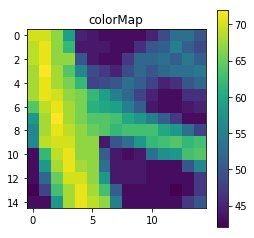
\includegraphics[width=0.5\textwidth]{images/noise.jpeg}
\caption[Ausschnitt der Lärmbelastung am Brausebad (Basel)]{Ausschnitt der Lärmbelastung am Brausebad (Basel)}
\label{fig:noise}
\end{figure}
\newline
%
Tabelle \ref{tab:fourth_round} zeigt die Ergebnisse, mit dem neuen Feature ‘Lärmbelastung’.\\[2ex]
%
\begin{table*}[ht]
\centering
\ra{1.3}
\resizebox{\textwidth}{!}{
\begin{tabular}{@{}lrrrrr@{}}
\toprule
ML Algorithmus & $R^2$ & MAPE & MdAPE & 10\% Abweichung & Maximaler Fehler\\
\midrule
Extra Tree & 0.838332 & 9.912 & 0.85 & 82.002 & 2.79E+07\\
XGBoost & 0.814466 & 9.952 & 0.74 & 82.212 & 2.81E+07\\
AdaBoost & 0.823295 & 9.954 & 0 & 83.593 & 2.75E+07\\
\bottomrule
\end{tabular}}
\caption{Ergebnisse mit Einbezug der Lärmbelastung}
\label{tab:fourth_round}
\end{table*}
%
Interessanter weise wurden die MAPE bei allen Modellen schlechter. Der Rest blieb etwa gleich. Jedoch hat das Feature vergleichsweise zur letzten Konstruktion eine höhere Gewichtung von 1.2\%.\\[2ex]
%
Auffallend bis jetzt bei allen Modellen war der hohe maximale Fehler zwischen 17 und 25 Millionen. Um diesen Fehler zu verkleinern führen wir vor dem Lernen eine Outlier Detection durch. Somit werden Immobilien mit nicht normalen Werten aus dem Datensatz entfernt.\\[2ex]
%
\textbf{Outlier Detection}\\
Für die Outlier Detection verwendeten wir einen Isolation Forest Algorithmus. Es werden nur die numerischen Features auf Ausreisser überprüft, da diese am Fehleranfälligsten sind.\\[2ex]
%
Beim Isolation Forest definiert ein Prozentsatz die Anzahl an markierten Outliers. 
Um einen geeigneten Prozentsatz zu bestimmen, vergleichen wir die entwicklung Standardabweichung beim erhöhen des Prozentsatz.\\
Ist die Differenz der Standardabweichung mit der Vorherigen nicht um mehr als 2.5\% gesunken, haben wir unseren optimalen Prozentsatz gefunden.\\
Abbildung \ref{fig:outlier} zeigt die Reduktion der Standardabweichung und die gefundenen Outlier bei der Wohnfläche. 
%
\begin{figure}[ht]
\begin{subfigure}{.5\textwidth}
  \centering
  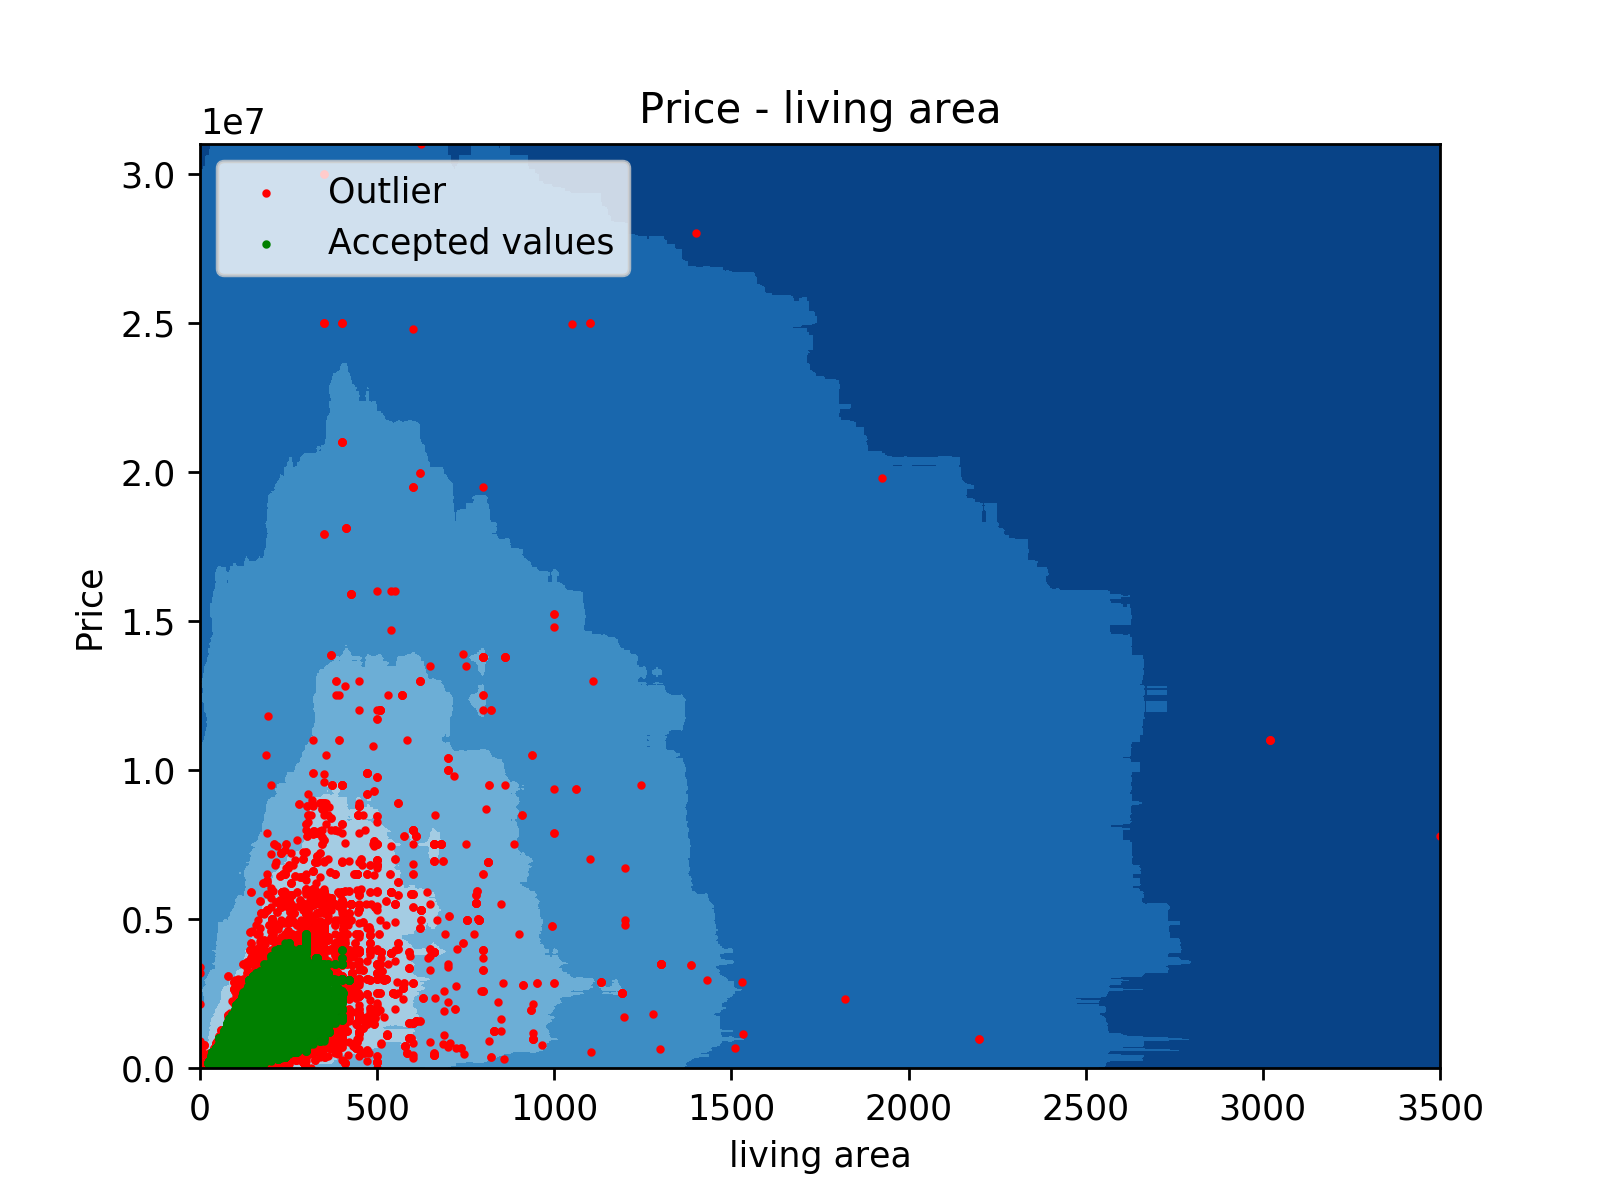
\includegraphics[width=\linewidth]{images/living_area_IsolationForest.png}
  \caption[Isolation Forest angewendet auf Wohnfläche]{Isolation Forest angewendet auf Wohnfläche}
  \label{fig:isolation_forest}
\end{subfigure}%
\begin{subfigure}{.5\textwidth}
  \centering
  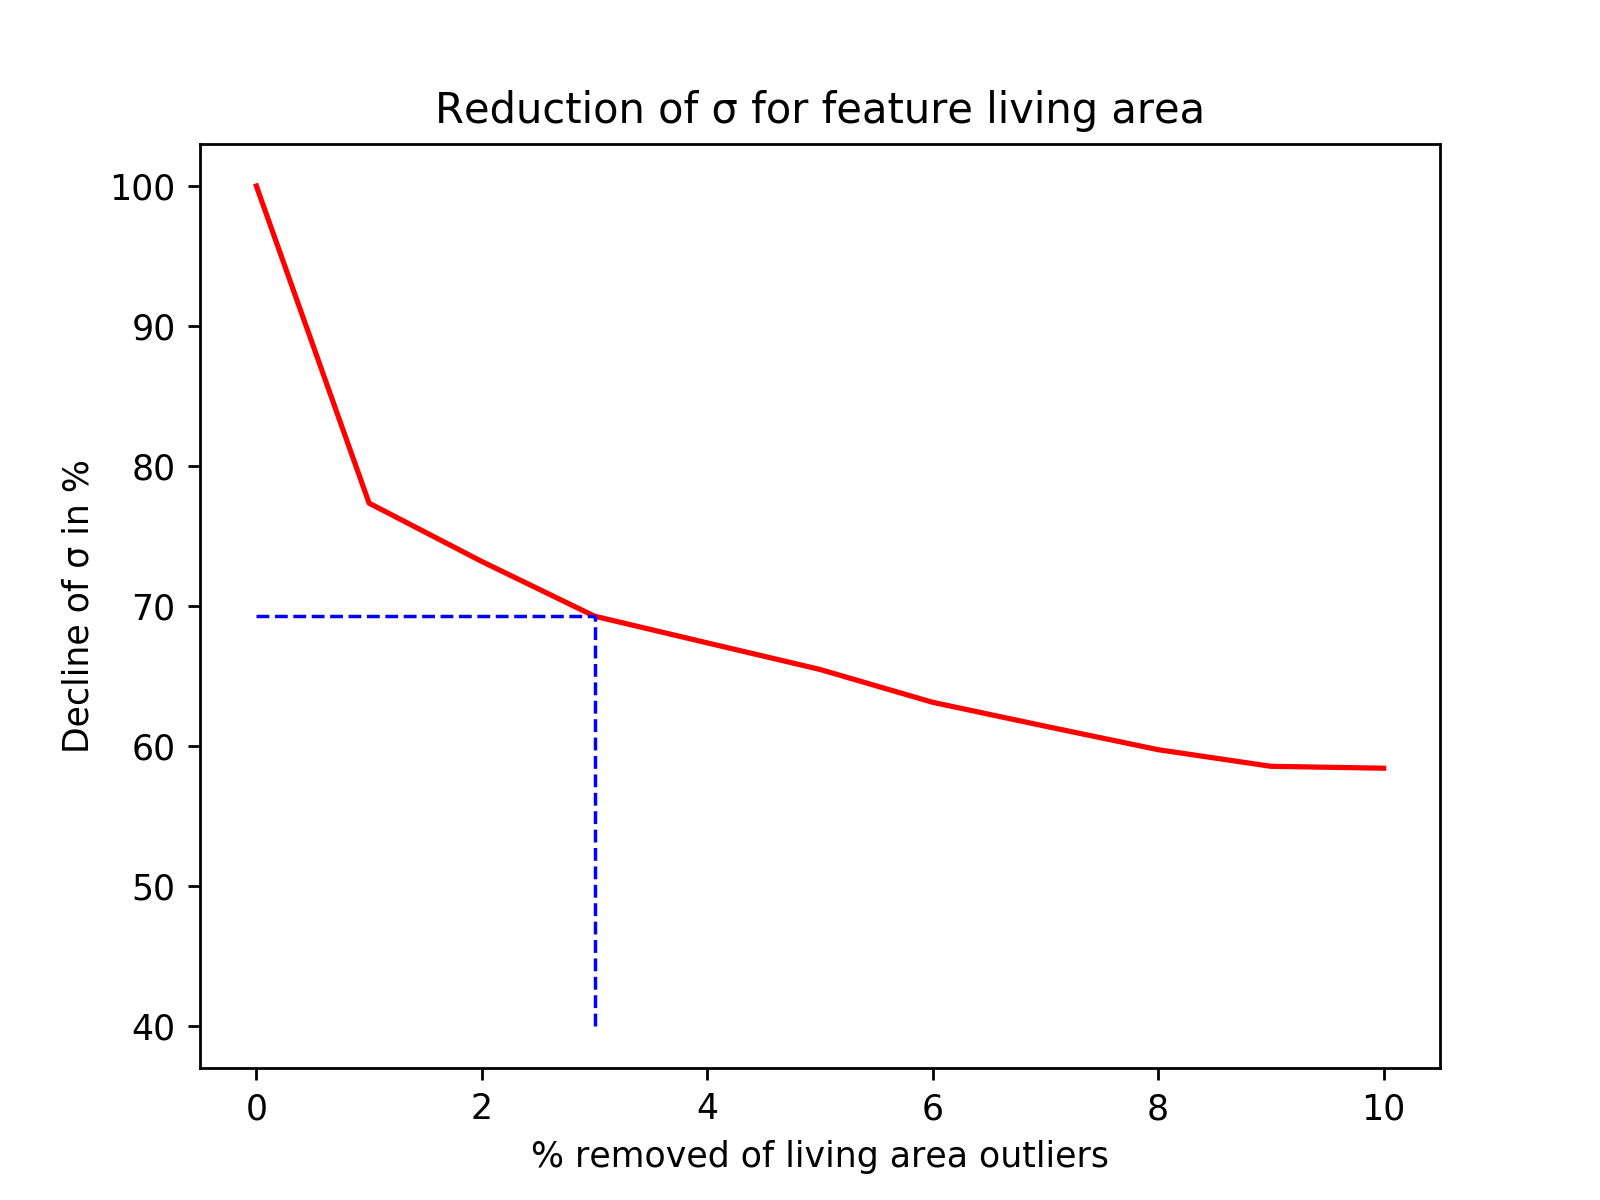
\includegraphics[width=\linewidth]{images/living_area_std.png}
  \caption[Entwicklung der Standardabweichung]{Entwicklung der Standardabweichung}
  \label{fig:}
\end{subfigure}
\caption[Outlier Detection: Wohnfläche]{Outlier Detection: Wohnfläche}
\label{fig:outlier}
\end{figure}
%
Die Outlier Detection wird nach dem Transformieren der Features ausgeführt. Tabelle \ref{tab:iso_forest} zeigt die gefunden Ausreisser im Datensatz. Insgesamt wurden 12'362 Inserate als Ausreisser markiert und entfernt.\\[2ex]
%
\begin{table*}[ht]
\centering
\ra{1.3}
\begin{tabular}{@{}lrr@{}}
\toprule
Feature & Entfernt in \% & \# entfernte Inserate\\
\midrule
Baujahr & 5 & 4293\\
Anzahl Zimmer & 3 & 2579\\
Wohnfläche & 3 & 2577\\
Letzte Konstruktion & 5 & 4294\\
Lärmbelastung & 7 & 7726\\
\bottomrule
\end{tabular}
\caption{Übersicht der Entfernten Inserate mit dem Isolation Forest}
\label{tab:iso_forest}
\end{table*}
%
Es ist unschwer zu erkennen, dass gewisse Inserate nicht nur bei einem Feature als Ausreisser markiert werden, sondern gleich bei mehreren.\\[2ex]
%
Betrachtet man die Einführung der Outlier Detection auf die Performance der Algorithmen in Tabelle \ref{tab:fifth_round}, sieht man, dass der Maximale Fehler auf 1 bis 1.7 Millionen verkleinert wurde.\\[2ex]
%
\begin{table*}[ht]
\centering
\ra{1.3}
\resizebox{\textwidth}{!}{
\begin{tabular}{@{}lrrrrr@{}}
\toprule
ML Algorithmus & $R^2$ & MAPE & MdAPE & 10\% Abweichung & Maximaler Fehler\\
\midrule
Extra Tree & 0.947074 & 5.216 & 0.702 & 84.269 & 1.89E+06\\
XGBoost & 0.941227 & 5.392 & 0.604 & 84.208 & 1.95E+06\\
AdaBoost &0.940529 & 4.692 & 0 & 85.609 & 1.95E+06\\
\bottomrule
\end{tabular}}
\caption{Ergebnisse mit Einbezug einer Outlier Detection}
\label{tab:fifth_round}
\end{table*}
%
Es zeigt sich, dass eine Outlier Detection wichtig ist. Der MAPE konnte um 10\% verbessert werden.\\[2ex] 
%
Interessant zu wissen, wäre ob der Steuersatz eine Auswirkung auf das Modell hat. Deshalb haben wir vom Bundesamt für Statistik der Gemeinde Steuerfuss wie auch der Kontonssteuerfuss beschafft und diesen in unser Modell miteinbezogen. Tablle \ref{tab:sixth_round} zeigt das Ergebnis.\\[2ex]
\begin{table*}[ht]
\centering
\ra{1.3}
\resizebox{\textwidth}{!}{
\begin{tabular}{@{}lrrrrr@{}}
\toprule
ML Algorithmus & $R^2$ & MAPE & MdAPE & 10\% Abweichung & Maximaler Fehler\\
\midrule
Extra Tree & 0.946107 & 5.39 & 0.686 & 83.799 & 1.55E+06\\
XGBoost & 0.940157 & 5.382 & 0.632 & 83.997 & 1.82E+06\\
AdaBoost &0.943958 & 4.64 & 0 & 85.596 & 1.81e+06\\
\bottomrule
\end{tabular}}
\caption{Ergebnisse mit Einbezug des Steuerfuss}
\label{tab:sixth_round}
\end{table*}
%
Unser Modell besitzt insgesamt 42 verschiedene Tags als Feature. Diese Tags beschreiben zum Teil dasselbe mit anderen Worten. Daher lohnt es sich aus mehreren schwachen Features ein starkes Feature zu bilden. Wir definieren 4 Gruppen die den Wert 1 besitzen, sobald ein Tag das zur Gruppe gehört vorhanden ist. Ansonsten ist es auf 0.
\begin{description}
\item[Badezimmer:] Alle Tags die eine Nasszelle beschreiben. Dazugehört Badezimmer, Lavabo, Dusche usw.
\item[Innenausstattung:] Alle Tags die eine Innenausstattung beschreiben wie TV Anschluss, gross, hell usw. 
\item[Aussenausstattung:] In diese Kategorie fallen Tags wie Garten, Balkon, Garage, Parkplatz usw.
\item[Nachbarschaft:] Beschreibt die Umgebung der Immobilie. Ist es zentral, ruhig, hat es Einkaufsmöglichkeiten usw.
\end{description}
%
\begin{table*}[ht]
\centering
\ra{1.3}
\resizebox{\textwidth}{!}{
\begin{tabular}{@{}lrrrrr@{}}
\toprule
ML Algorithmus & $R^2$ & MAPE & MdAPE & 10\% Abweichung & Maximaler Fehler\\
\midrule
Extra Tree & 0.947874 & 4.854 & 0.109 & 85.541 & 2.54E+06\\
XGBoost &0.945822 & 4.881 & 0.074 & 85.759 & 2.50E+06\\
AdaBoost &0.93973 & 4.544 & 0 & 86.317 & 2.60E+06\\
\bottomrule
\end{tabular}}
\caption{Ergebnisse mit gruppierten Tags}
\label{tab:seventh_round}
\end{table*}
%
Viel verändert hat sich nicht. Obwohl die Zeit für die Berechnung der einzelnen Modelle schneller ging. Somit lohnt es sich eventuell auch weitere Features die keine Gewichtung besitzen vor dem berechnen zu löschen.\\[2ex]
%
Wir möchten noch wissen wie wichtig die Ortsbezogenen Features vom BFS sind. Dafür erstellen wir ein Modell, das nur aus den gesammelten Daten von den Plattformen erstellt wird.
Tabelle zeigt die Resultate dieser berechnung.\\[2ex]
%
\begin{table*}[ht]
\centering
\ra{1.3}
\resizebox{\textwidth}{!}{
\begin{tabular}{@{}lrrrrr@{}}
\toprule
ML Algorithmus & $R^2$ & MAPE & MdAPE & 10\% Abweichung & Maximaler Fehler\\
\midrule
Extra Tree & 0.907327 & 7.092 & 0.684 & 79.063 & 1.96E+06\\
XGBoost & 0.892067 & 8.692 & 0.941 & 78.207 & 2.16E+06\\
AdaBoost & 0.893971 & 7.054 & 0 & 80.176 & 1.96E+06\\
\bottomrule
\end{tabular}}
\caption{Ergebnisse ohne ortsbezogenen Daten vom BFS}
\label{tab:height_round}
\end{table*}
%
\subsubsection{Kombinierte Algorithmen}
Als weiteren Test haben wir einen eigenen Regressor erstellt, der mehrere Machine Learnig Algorithmen kombiniert.\\[2ex]
%
Dieser Algorithmus hat im Endeffekt zwei Schätzphasen. Zunächst wird ein Extra Tree trainiert, und für jeden Train-Datensatz werden alle Decision Pathes für alle Bäume abgespeichert. Um nun eine Schätzung zu erhalten, werden zuerst die Decision Pathes für den zu testenden Datensatz herausgesucht, und mit den Train-Datensätzen verglichen. Alle Train-Datensätze mit mindestens einem passendem Decision Path werden markiert für die zweite Phase der Schätzung.\\
In der zweiten Phase werden diese markierten Datensätze auf einem weiteren Machine Learning Algorithmus ad-hoc trainiert. Der zweite Algorithmus kann nach beliben ausgetauscht werden. Anschliessend wird auf diesem neuen Model der Test-Datensatz geschätzt.\\
Theoretisch wäre es möglich für alle möglichen Decision Pathes die Models im Vorhinein zu berechnen, da nur eine finite Anzahl an Decision Pathes existieren. Dies ist aber aus praktikablen Gründen nicht möglich, da mit vielen Datensätzen die trainierten Bäume gross werden und entsprechend  dafür zu viel RAM und Rechenzeit benötigt wird.\\[2ex]
%
Um genügend Datensätze für die zweite Phase zu erhalten, wird der Extra Tree mit einer minimalen Leaf Size von fünf Samples konfiguriert.\\
Für den zweiten Schätzungsalgorithmus verwenden wir den K-Nearest Neighbour wie oben beschrieben.
%
\begin{table*}[ht]
\centering
\ra{1.3}
\resizebox{\textwidth}{!}{
\begin{tabular}{@{}lrrrrr@{}}
\toprule
ML Algorithmus & $R^2$ & MAPE & MdAPE & 10\% Abweichung & Maximaler Fehler\\
\midrule
Extra Tree mit KNN & 43.636 & 13.451 & 40.034 &  0.619114 & 2.94294e+07\\
\bottomrule
\end{tabular}}
\caption{Ergebnisse ohne ortsbezogenen Daten vom BFS}
\label{tab:combined}
\end{table*}
%
Wie man in Tabelle \ref{tab:combined} sieht, waren die Ergebnisse weitaus schlechter als oben verwendete Algorithmen. Wir können uns dieses Verhalten nicht erklären. Weitere Forschunten konnten nicht durchgeführt werden, da uns für das die Zeit fehlte.\\[2ex]
%
Als letztes kombinieren wir noch die drei Baumalgorithmen miteinander. Da der AdaBoost immer ein bisschen besser war als die anderen beiden, erhält dieser mehr gewicht für die Schätzung. Das Resultat konnte doch noch verbessert werden, wie Tabelle \ref{tab:combined_2} zeigt.\\
Hierfür wurden dem AdaBoost 0.8, dem XGBoost 0.2 und dem Extra Tree 0.1  Gewichtung gegeben.
%
\begin{table*}[ht]
\centering
\ra{1.3}
\resizebox{\textwidth}{!}{
\begin{tabular}{@{}lrrrrr@{}}
\toprule
ML Algorithmus & $R^2$ & MAPE & MdAPE & 10\% Abweichung & Maximaler Fehler\\
\midrule
Kombiniert & 0.94646 & 4.416 & 0.07 & 87.03	& 1.77E+06\\
\bottomrule
\end{tabular}}
\caption{Ergebnisse ohne ortsbezogenen Daten vom BFS}
\label{tab:combined_2}
\end{table*}
%
\subsection{Auswertung}
Es hat sich gezeigt, dass eine Kombination des AdaBoost, Extra Tree und XGBoost die besten Resultate erzielt. Betrachtet man die Algorithmen alleine hatte bei unseren Daten der AdaBoost die besten Ergebnisse.\\ 
Von der Berechnungszeit ist der AdaBoost klar der Beste, da dieser für ein Fit ungefähr 10 Minuten benötigt, während er XGBoost under der Extra Tree über eine Stunde benötigen.\\
Wir konnten mit unserer eigenen Implementation eines Machine Learning Algorithmus keinen Erfolg erzielen, da die Performance nicht zufriedenstellend war.\\[2ex]
%
Weiter konnte bewiesen werden, dass sich ein ausgiebiges Feature Engineering auf die Performance positiv auswirkt. Vor allem eine Outlier Detection kann das Modell um 10\% verbessern. Der Versuch seltene Features so zu transformieren, dass man sie verwenden kann, hilft auch um eine bessere Performance zu erhalten. \\
Es ist Sinnvoll ortsbezogene Daten als Features zu verwenden. Mit diesen Features konnte eine Steigerung von 4\% bei den richtig Geschätzten Immobilien erzielt werden. Das zeigt, dass der Preis nicht nur von der Immobilie sondern auch vom Standort abhängig ist. \\[2ex]
%
Auch wenn die öffentlichen Daten von Immobilien eine eher schlechte Qualität besitzen, reichen sie aus für ein gutes Schätzungsmodell. Insgesamt konnten 85’845 von 162’225 verwendet werden. Die meisten Inserate konnten nicht verwendet werden, da sie keine Angaben über wichtige Kennwerte hatten.

subsection{Gültigkeitsrisiken}
Man muss bedenken, dass wir unsere Modelle auf geschätzten Werten trainiert haben. Somit ist der geschätzte Wert mit Vorsicht zu betrachten. Auch ist der Immobilienpreis immer gewissen Schwankungen ausgesetzt sodass dieser in einem halben Jahr schon wieder anderst ist.\\
Wir haben die Kennwerte von öffentlichen Immobilienplattformen gesammelt. Es geht dort hauptsächlich darum die Immobilie zu verkaufen. So wird auch gerne mal ein bisschen geschummelt, schöngeredet oder die Angaben der Kennwerte werden falsch eingetragen. Eine Outlier Detection kann nur grobe Ausreisser erkennen. Kleinere Ausreisser bleiben somit unentdeckt und können das Modell verfälschen.\\
Wird eine neue Siedlung oder ein neuer Wohnblock inseriert, kann es vorkommen, dass 10 mal die gleiche Wohnung inseriert wird. Dies ist unschön, da diese Wohnungen mehr Gewicht erhalten.

